%\documentclass{article}
%\documentclass[draft]{report}%{article}
\documentclass{report}%{article}
\usepackage{graphicx}
%\usepackage[draft]{graphicx}
\graphicspath{{figs}{notebooks}{.}}
\usepackage{hyperref}
\usepackage{amsmath}
\usepackage{amsfonts}
\usepackage{amssymb}
\usepackage[margin=1in]{geometry}
\usepackage{comment}
\usepackage{color}
\usepackage[acronym]{glossaries}
%\usepackage{alphalph} % For extended alphabetical numbering
\usepackage{appendix}

% \usepackage[%
%filename ,%
%content={no image available}
%]{draftfigure}

\makeglossaries
% \newacronym{label}{acronym}{definition}

\newacronym{TFT}{TFT}{Thin-Film Transistor}
\newacronym{TFT}{TFT}{GastroIntestinal}

\newacronym{LM}{LM}{Light Microscopy}
\newacronym{EM}{EM}{Electron Microscopy}
\newacronym{TEM}{TEM}{Transmission Electron Microscopy}
\newacronym{SEM}{SEM}{Scanning Electron Microscopy}
\newacronym{SPM}{SPM}{Scanning Probe Microscopy}
\newacronym{AFM}{AFM}{Atomic Force Microscopy}
\newacronym{STM}{STM}{Scanning Tunneling Microscope}

\newacronym{ET}{ET}{Electron Tomography}
\newacronym{cryo-ET}{Cryo-ET}{Cryo-Electron Tomography}
\newacronym{OPT}{OPT}{Optical Projection Tomography}
\newacronym{SXT}{STX}{Soft X-ray Tomography}
\newacronym{PAT}{PAT}{PhotoAcoustic Tomography}

\newacronym{GT}{GT}{Ground Truth}

\newacronym{DRV}{DRV}{Discrete Random Variable}

\newacronym{CC}{CC}{Cross-Correlation}
\newacronym{NCC}{NCC}{Normalized Cross-Correlation}
\newacronym{PCC}{PCC}{Pearson Correlation Coefficient}
\newacronym{AC}{AC}{Auto-Correlation}
\newacronym{NAC}{NAC}{Normalized Auto-Correlation}
\newacronym{SNR}{SNR}{Signal-to-Noise Ratio}
\newacronym{PSNR}{PSNR}{Peak \acrshort{SNR}}
\newacronym{SSNR}{SSNR}{Spectral Signal-to-Noise Ratio}
\newacronym{SRV}{SRV}{Stationary Random Variable}
\newacronym{FTDF}{FTDF}{Fourier Transform of a Discrete Function}
\newacronym{DTFT}{DTFT}{Discrete Time Fourier Transform}
\newacronym{IDTFT}{IDTFT}{Inverse Discrete Time Fourier Transform}
\newacronym{DFT}{DFT}{Discrete Fourier Transform}
\newacronym{IDFT}{IDFT}{Inverse Discrete Fourier Transform}
\newacronym{FFT}{FFT}{Fast Fourier Transform}
\newacronym{IFFT}{IFFT}{Inverse Fast Fourier Transform}
\newacronym{PS}{PS}{Power Spectrum}
\newacronym{PSD}{PSD}{Power Spectral Density}
\newacronym{CPSD}{CPSD}{Cross-Power Spectral Density}
\newacronym{MAD}{MAD}{Mean Absolute Deviation}

\newacronym{AWG}{AWG}{Additive White Gaussian}
\newacronym{PDF}{PDF}{Probability Density Function}
\newacronym{PMF}{PMF}{Probability Mass Function}
\newacronym{PMD}{PMD}{Probability Mass Distribution}
\newacronym{MPG}{MPG}{Mixed Poisson-Gaussian}

\newacronym{FSC}{FSC}{\href{https://en.wikipedia.org/wiki/Fourier_shell_correlation}
{Fourier Shell Correlation}}
\newacronym{SFRC}{SFRC}{Self Fourier Ring Correlation}
\newacronym{FRC}{FRC}{Fourier Ring Correlation}
\newacronym{FC}{FC}{Fourier Correlation}
\newacronym{SFC}{SFC}{Self Fourier Correlation}

\newacronym{DOF}{DOF}{Dense Optical Flow}
\newacronym{EOS}{EOS}{Even-Odd Splitting}
\newacronym{CBS}{CBS}{ChessBoard Splitting}
\newacronym{ICBS}{ICBS}{Interpolated \acrshort{CBS}}
\newacronym{SCBS}{SCBS}{Subsampled \acrshort{CBS}}
\newacronym{SPRS}{SPRS}{Structure Preserving Random Shuffling}
\newacronym{TRPR}{TRPR}{TriS-D Random Pixel Resampling}

\newacronym{MSE}{MSE}{Mean Square Error}
\newacronym{RMSE}{RMSE}{Root \acrshort{MSE}}
\newacronym{SSIM}{SSIM}{Structural Similarity Index Measure }
\newacronym{MS-SSIM}{MS-SSIM}{Multi-Scale \acrshort{SSIM}}
\newacronym{LPIPS}{LPIPS}{Learned Perceptual Image Patch Similarity}
\newacronym{NIQE}{NIQE}{Natural Image Quality Evaluator}
\newacronym{CS}{CS}{Cosine Similarity}

\newacronym{CLT}{CLT}{Central Limit Theorem}
\newacronym{GAT}{GAT}{Generalized Anscombe Transform}
\newacronym{VST}{VST}{Variance-Stabilizing Transform}
\newacronym{MNI}{MNI}{Mean of Noisy Instances}

\newacronym{GF}{GF}{Gaussian Filtering}
\newacronym{WF}{WF}{Wiener Filtering}
\newacronym{GD}{GD}{Gaussian Denoising}
\newacronym{TF}{TF}{Transfer Function}
\newacronym{LTI}{LTI}{Linear Time-Invariant}
\newacronym{NoO}{NoO}{Number of Operations}
\newacronym{IIR}{IIR}{Infinite Impulse Response}
\newacronym{FIR}{IIR}{Finite Impulse Response}

\newacronym{CNN}{CNN}{Convolutional Neural Network}

\newacronym{BM3D}{BM3D}{Block-Matching and 3D filtering}
\newacronym{DnCNN}{DnCNN}{Denoising \acrshort{CNN}}

\title{Denoising in Microscopy Imaging}

\author{Vicente González-Ruiz and José Jesús Fernández Rodríguez}

\begin{document}
\maketitle
\tableofcontents

\section*{Definitions and notation}
%{{{

\begin{tabular}{ll}
  $x$ & A scalar value (e.g., a value of a pixel of a grayscale image) \\
  $s(t)$ & A (continuous) signal as a function of time \\
  $s[n]$ & A discrete signal (only) defined at instants of time $tn, n\in\mathcal{Z}, t>0$ \\
  $\mathbf{s}$ & A digital (discrete and finite) signal (e.g., an image) \\
  $\mathbf{s}_{i}$ & The $i$-th element of $\mathbf{s}=\{\mathbf{s}_{i}\}_{i=0}^{N-1}=\{\mathbf{s}_{i}\}$ \\
  %$A[b]$ & The $b$-th element of the sampled version of $A(b)$ \\
  $\{i\}$ & The set $i$ \\
  $\mathbf{s}_{\{i\}}$ & The elements of $\mathbf{s}$ with indices $\{i\}$ \\
  $\mathbf{s}_{[i]}$ & A window of samples of $\mathbf{s}$ centered at the $i$-th sample \\
  $\mathbf{s}_{\href{https://numpy.org/doc/stable/user/basics.indexing.html#slicing-and-striding}{y,:}}$ & The $y$-th row of the image $\mathbf{s}$ \\
  $\mathbf{s}_{:,x}$ & The $x$-th column of the image $\mathbf{s}$ \\
  $\mathbf{s}_{y,x}$ & The pixel $(y,x)$ of the image $\mathbf{s}$ \\
  %$\mathbf{x}^{(i)}$ & The $i$-th real-noisy instance of the signal $\mathbf{x}$ \\
  %$\mathbf{s}^{()}$ & An instance of $\mathbf{s}$, possibly noisy \\
  $\mathbf{s}^{(i)}$ & The $i$-th instance of the signal $\mathbf{s}$ \\
  $\tilde{\mathbf{s}}^{(I)}$ & Approximation to $\mathbf{s}$ using $I$ instances \\ 
  $\overline{\mathbf{s}}$ & A mean of the samples of $\mathbf{s}$ \\ 
  $\href{https://docs.python.org/3/library/functions.html#len}{\text{len}}(\mathbf{s})$ & $=\mathbf{s}.\href{https://numpy.org/doc/stable/reference/generated/numpy.ndarray.size.html}{\mathsf{size}}$ Number of elements in $\mathbf{s}$ \\
  $\href{https://numpy.org/doc/stable/reference/generated/numpy.shape.html}{\text{shape}}(\mathbf{s})$ & ($=\mathbf{s}.{\mathsf{shape}}$) Shape of $\mathbf{s}$ \\
  $\text{rank}(\mathbf{s})$ & ($=\mathbf{s}.\mathsf{rank}=\text{len}(\mathbf{s}.\mathsf{shape})$) Dimensionality of $\mathbf{s}$ \\
  $\mathsf{\href{https://docs.python.org/3/library/functions.html\#func-range}{range}}(s)$ & $=\{0, 1, \cdots, s-1\}$ \\
  $\mathsf{\href{https://numpy.org/doc/stable/reference/generated/numpy.zeros_like.html}{zeros\_like}}(\mathbf{s})$ & $=\{0\}_{i=0}^{\mathbf{s}.\mathsf{size}-1}$ \\
  % $|\mathbf{X}_i|$ & The absolute value of $\mathbf{X}_i$ \\
  $\alpha\mathbf{s}$ & $=\{\alpha\mathbf{s}_i\}$ (scalar multiplication) \\
  $\mathbf{x}+\mathbf{y}$ & $=\{\mathbf{x}_i + \mathbf{y}_i\}$ (Hadamard addition) \\ 
  $\mathbf{x}\mathbf{y}$ & $=\{\mathbf{x}_i\mathbf{y}_i\}$ (Hadamard product) \\ 
  $\mathcal{N}$ & The normal distribution \\ 
  $\mathcal{P}$ & The Poisson distribution \\
  $\mathbf{x}\sim\mathcal{N}$ & The elements of $\mathbf{x}$ follows a normal distribution \\
  $\mathbf{x}_{\mathcal{N}}$ & The same as $\mathbf{x}\sim\mathcal{N}$ \\
  $\Pr(\mathbf{x}=a)$ & Probability that a $\mathbf{x}_i$ takes the value $a$ \\
  $\Pr(\mathbf{x}=a, \mathbf{y}=b)$ & $\Pr(\mathbf{x}=a)$ and $\Pr(\mathbf{y}=b)$ (joint probability)  \\
  $\text{Su}(\mathbf{x})$ & $=\{x\in\mathbb{R}|\Pr(\mathbf{x}=x)>0\}$ (support of $\mathbf{x}$)\\
  $\Pr(A|B)$ & Conditional probability of $A$ given $B$ \\
  $\mathbb{E}(\mathbf{s})$ & Expectation of $\mathbf{s}$ \\
  $\mathbb{V}(\mathbf{s})$ & Variance of $\mathbf{s}$ \\
  $||\mathbf{s}||_2$ & $L_2$ norm of $\mathbf{s}$ \\
  $f_s$ & Sampling frequency \\
  $\mathcal{F}$ & The (forward) Fourier transform ($\mathcal{F}(\mathbf{s})=\mathbf{S}$) (see Section~\ref{sec:Fourier_transform})\\
  $\mathcal{F}^{-1}$ & The inverse Fourier transform ($\mathcal{F}^{-1}(\mathbf{S})=\mathbf{s}$)  (see Section~\ref{sec:Fourier_transform})\\
  $\cdot^*$ & the complex conjugate of $\cdot$ \\
  $\mathbf{x}*\mathbf{y}$ & $=\mathcal{F}^{-1}(\mathcal{F}(\mathbf{x})\mathcal{F}(\mathbf{y}))=\mathcal{F}^{-1}(\mathbf{X}\mathbf{Y})$ (convolution) \\
  $A(b)$ & $A$ depends on (parameter) $b$ \\
  $A.b$ & The $b$ component of the data structure $A$ \\
  $(A)b$ & First $A$, then $b$ \\
  $E(\mathbf{s})$ & Energy of $\mathbf{s}$ (see Section~\ref{sec:energy_signal}) \\
  $P(\mathbf{s})$ & Power of $\mathbf{s}$ (see Section~\ref{sec:power_signal}) \\
  $\text{PS}(\mathbf{s})$ & Power spectrum of $\mathbf{s}$ (see Section~\ref{sec:power_spectrum}) \\
  $\text{PSD}(\mathbf{s})$ & Power spectral density of $\mathbf{s}$ (see Section~\ref{sec:PSD}) \\
  $\text{CC}(\mathbf{x},\mathbf{y})$ & Cross-correlation between $\mathbf{x}$ and $\mathbf{y}$ (see Section~\ref{sec:cross-correlation}) \\
  $\text{NCC}(\mathbf{x},\mathbf{y})$ & Normalized cross-correlation between $\mathbf{x}$ and $\mathbf{y}$ (see Section~\ref{sec:cross-correlation}) \\
  $\mathbf{a}\bot \mathbf{b}$ & $\mathbf{a}$ and $\mathbf{b}$ are orthogonal or independent                                
\end{tabular}

%}}}

\chapter{Image acquisition}
% Medical Image Acquisition

With the exception of nuclear medicine\footnote{In nuclear medicine
  imaging, radioactive substances are injected or ingested, and it is
  the physiological interactions of the agent that give rise to the
  information in the images \cite{bushberg2011essential}.}, all
medical imaging techniques require that the energy used to penetrate
the body’s tissues also interacts with those tissues.\footnote{If
  energy were to pass through the body and not experience some type of
  interaction (e.g., absorption or scattering), then the detected
  energy would not contain any useful information regarding the
  internal anatomy, and thus it would not be possible to construct an
  image of the anatomy using that information
  \cite{bushberg2011essential}.}

The power, energy and time required to acquiring medical images
require a compromise between patient safety and image
quality.\footnote{Better x-ray images can be made when the radiation
  dose to the patient is high, better magnetic resonance images can be
  made when the image acquisition time is long, and better ultrasound
  images result when the ultrasound power levels are large
  \cite{bushberg2011essential}.}



\section{Ultrasound}
\chapter{Ultrasound}
\vspace{-40ex}\hspace{35ex}
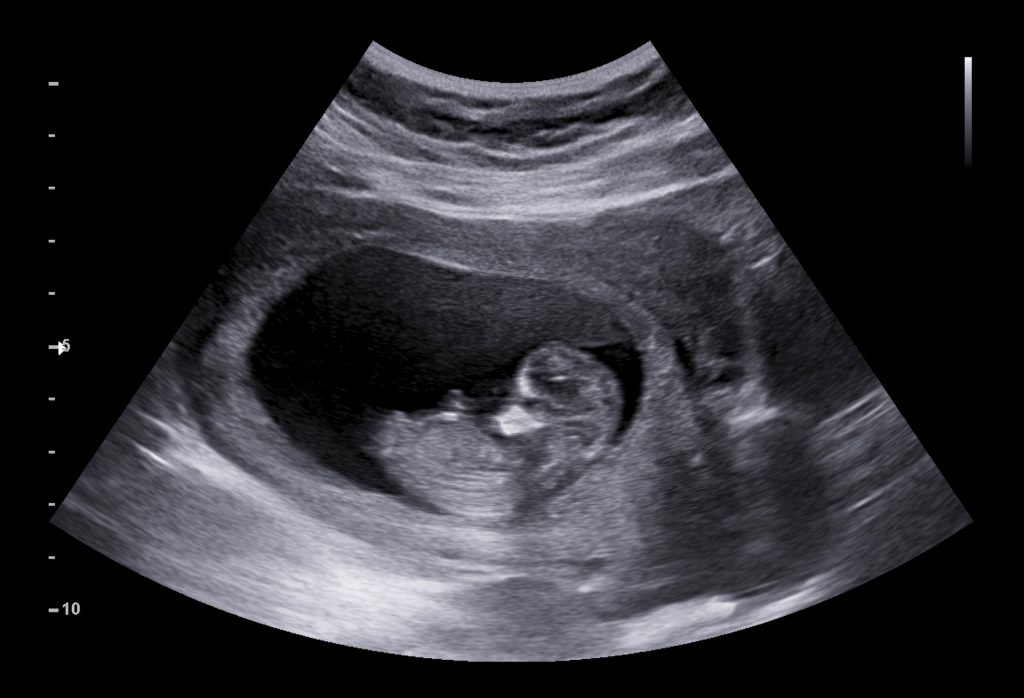
\includegraphics[width=10cm]{fetus_2D}

\section{Properties of sound}

\begin{itemize}
\item Mechanical energy in the form of \popup{high-frequency}{The
    higher the frequency the better resolution and image detail, but
    lower penetration.} (usually in the range of 2 to 18 MHz
  \cite{abdulla2025sound}) \popup{sound waves}{Sound waves are
    longitudinal preasure mechanical waves. They need a medium to
    propagate at a speed that depends on the rigidity and density of
    the medium. The typical speed in the tissue is 1540 m/s.} can be
  used to generate images of the anatomy of a patient (see Figure
  \ref{fig:sound}).
\end{itemize}
%\vspace{-2ex}
\begin{figure}[!h]
  \centering
  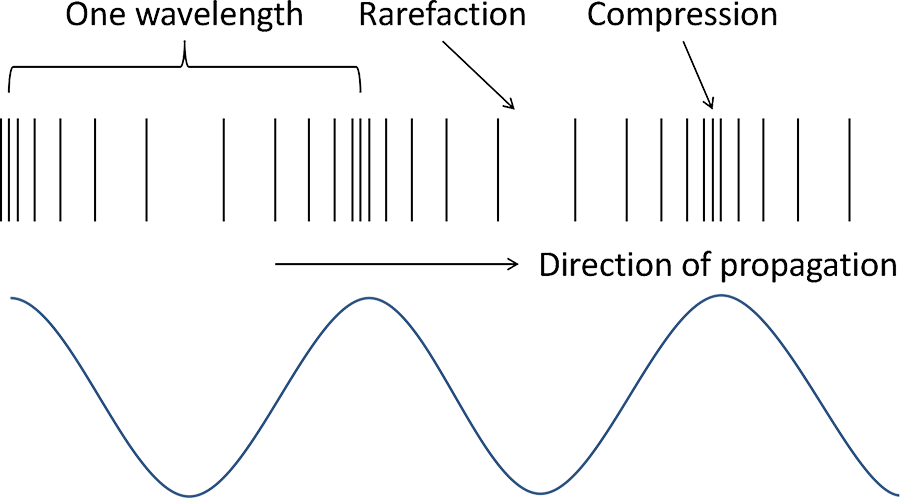
\includegraphics[width=8cm]{sound}
  \caption{Mechanical movement of the particles with the sound
    \cite{abdulla2025properties_sound}.\label{fig:sound}}
\end{figure}

\section{Echoes}
\begin{itemize}
\item \popup{(Ultra)Sound waves}{In form of decaying pulses.} pass
  through tissues, get reflected, and the returning wave (echo) is
  detected and forms the
  image\cite{bushberg2011essential,abdulla2025ultrasound_machine}. In
  \popup{B-mode}{B for Brightness (the most common ultrasound imaging
    used in medicine). There is A-Mode (A for Amplitude) that is
    mainly used in ophthalmology to investigate retinal detachment.}
  imaging, the intensity of the returning wave (echo) is represented
  as a level of brightness on the monitor to give a 2D cross-sectional
  image on the monitor \cite{abdulla2025ultrasound} (see Figure
  \ref{fig:interactions}).
\end{itemize}
%\vspace{-3ex}
\begin{figure}[!h]
  \centering
  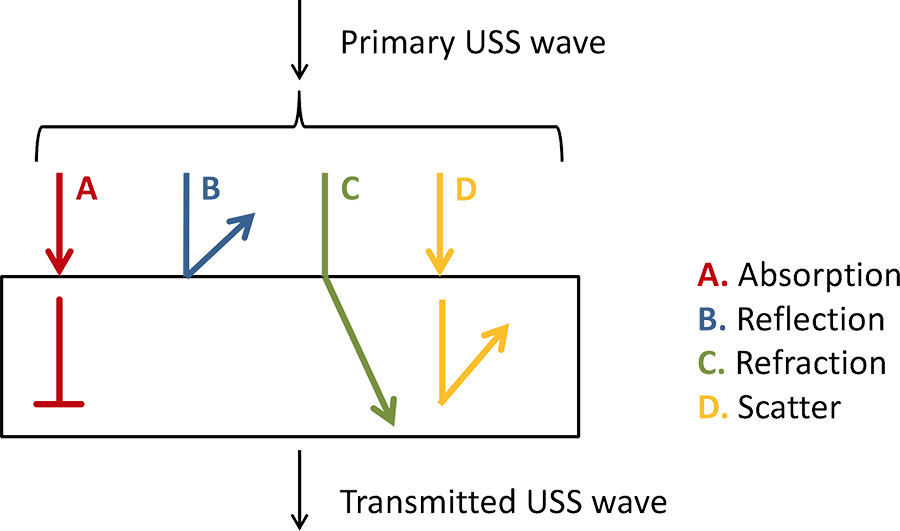
\includegraphics[width=7cm]{sound_interactions}
  \caption{Interactions of the ultrasound scan (USS) with tissue
    \cite{abdulla2025properties_sound}.\label{fig:interactions}}
\end{figure}

\section{Ultrasound imaging with flow detection}
\begin{itemize}
\item It is possible to use the \popup{M-Mode}{M for Motion.} (based
  on the Doppler effect) to detect the motion of fluids and mobile
  structures
  \cite{bushberg2011essential,abdulla2025ultrasound_machine}. Thus,
  for example, we can \popup{measure the blood flow}{Both the speed
    and direction of blood flow can be measured, and within a subarea
    of the grayscale image, a color flow display typically shows blood
    flow in one direction as red, and in the other direction as
    blue.}, displayed as color channels \cite{bushberg2011essential}
  (see Figure~\ref{fig:doppler}).
\end{itemize}
%\vspace{-4ex}
\begin{figure}[!h]
  \centering
  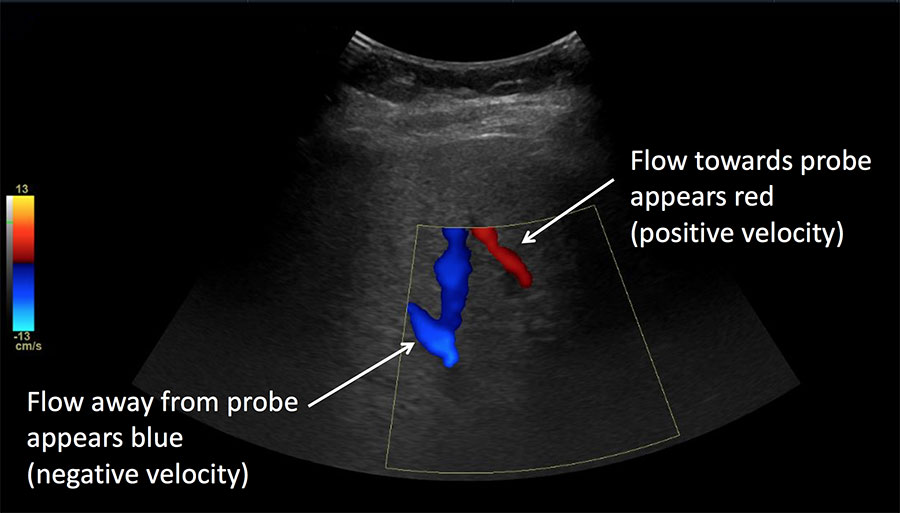
\includegraphics[width=8.0cm]{doppler}
  \caption{Ultrasound image showing flood motion
    \cite{abdulla2025ultrasound_imaging_doppler}.\label{fig:doppler}}
\end{figure}

\section{3D rendering}
\begin{itemize}
\item Ultrasound imaging is basically a \popup{2D technique}{By
    default, an ultrasound machine shows a deformed slice of the
    structure to analyze.}. However, 3D images can be generated by
  placing the known voxels in a
  \href{https://stackoverflow.com/questions/51907238/how-to-draw-a-2d-3d-grid-from-buffergeometry-in-three-js}{3D
    grid},
  \href{https://en.wikipedia.org/wiki/Trilinear_interpolation}{interpolating}
  the unknown voxels, and then,
  \href{https://en.wikipedia.org/wiki/Image_segmentation}{segmenting}
  (see Figure~\ref{fig:fetus_3D}).
\end{itemize}
%\vspace{-4ex}
\begin{figure}[!h]
  \centering
  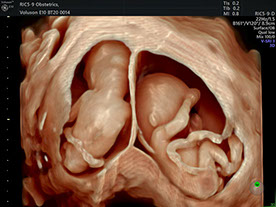
\includegraphics[width=6.0cm]{fetus_3D}
  \caption{3D ultrasound reconstruction
    \cite{fetal_diagnostic_centers}.\label{fig:fetus_3D}}
\end{figure}

\section{Artifacts}
\begin{itemize}
\item Image formation assumes that sound travels in straight lines, at
  a constant velocity, with uniform attenuation, and reflected only
  once from each interface \cite{abdulla2025ultrasound_artefacts}.
\item \popup{Artefacts}{Or artifacts, depending where you live!}
  result when the echo does not behave in this way and the system
  misinterprets it.
\end{itemize}

\section*{}
\subsection{Enhancement}
\begin{itemize}
\item Fluid filled structures are weakly
  \popup{attenuated}{Consequently, a larger proportion and greater
    amplitude beam passes through to structures in the region behind},
  and the image reconstruction algorithm interprets this as an
  \popup{increase in acoustic reflection}{The structures below show up
    brighter on the image.} (see
  Figure~\ref{fig:acoustic_enhancement}).
\end{itemize}
%\vspace{-3ex}
\begin{figure}[!h]
  \centering
  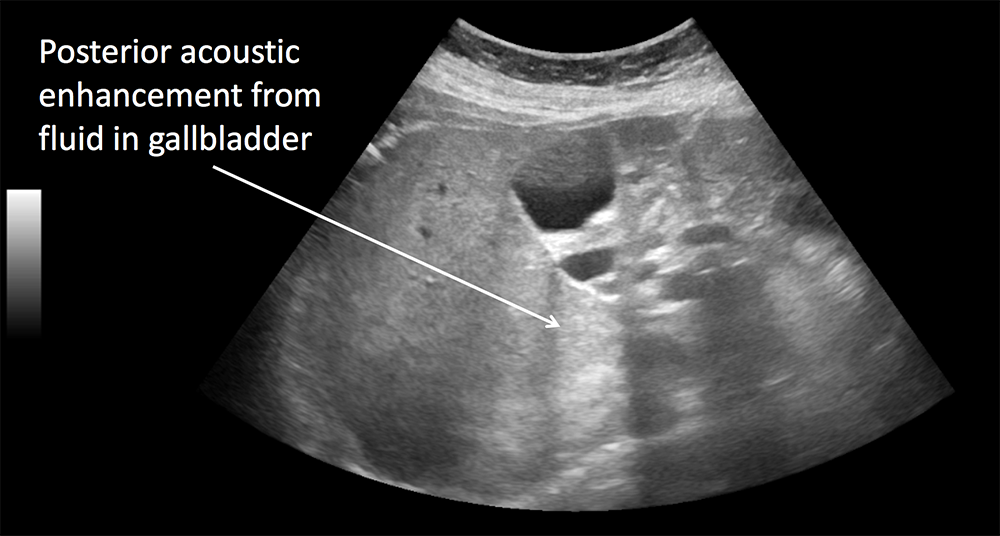
\includegraphics[width=8cm]{acoustic_enhancement}
  \caption{Acoustic enhancement artefact in ultrasound
    \cite{abdulla2025ultrasound_artefacts}.\label{fig:acoustic_enhancement}}
\end{figure}

\section*{}
\subsection{Shadowing}
\begin{itemize}
\item Hard calcific substances and soft tissue-air interfaces reflect almost all of the soundwaves. Therefore, no information is received from the area behind the structure (see
  Figure~\ref{fig:acoustic_shadowing}).
\end{itemize}
\vspace{-1ex}
\begin{figure}[!h]
  \centering
  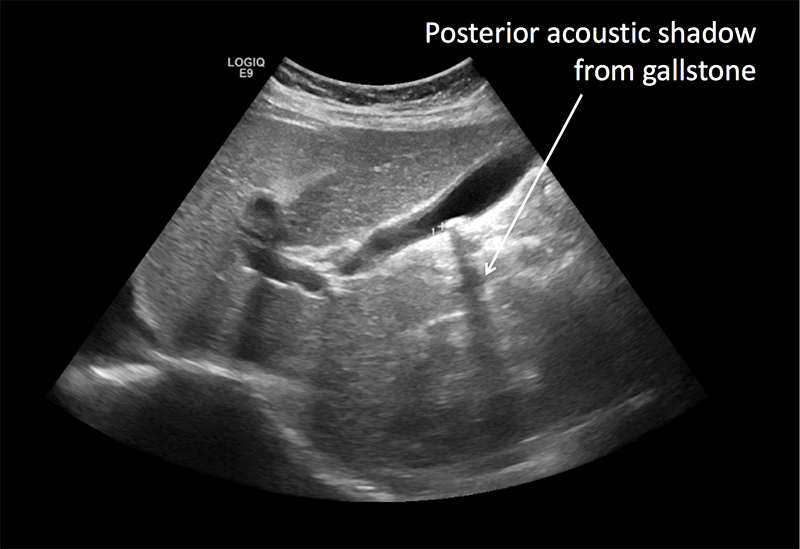
\includegraphics[width=6.5cm]{acoustic_shadowing}
  \caption{Acoustic shadowing artefact in ultrasound
    \cite{abdulla2025ultrasound_artefacts}.\label{fig:acoustic_shadowing}}
\end{figure}

\section*{}
\subsection{Reverberation}
\begin{itemize}
\item Reverberation artifacts occur when sound waves bounce back and
  forth between two surfaces, creating \popup{multiple echoes}{These
    echoes appear as parallel lines on the image, giving the
    appearance of multiple objects or structures.}. (see
  Figure~\ref{fig:acoustic_reverberation}) \cite{NysoraArtifacts}.
\end{itemize}
\vspace{-1ex}
\begin{figure}[!h]
  \centering
  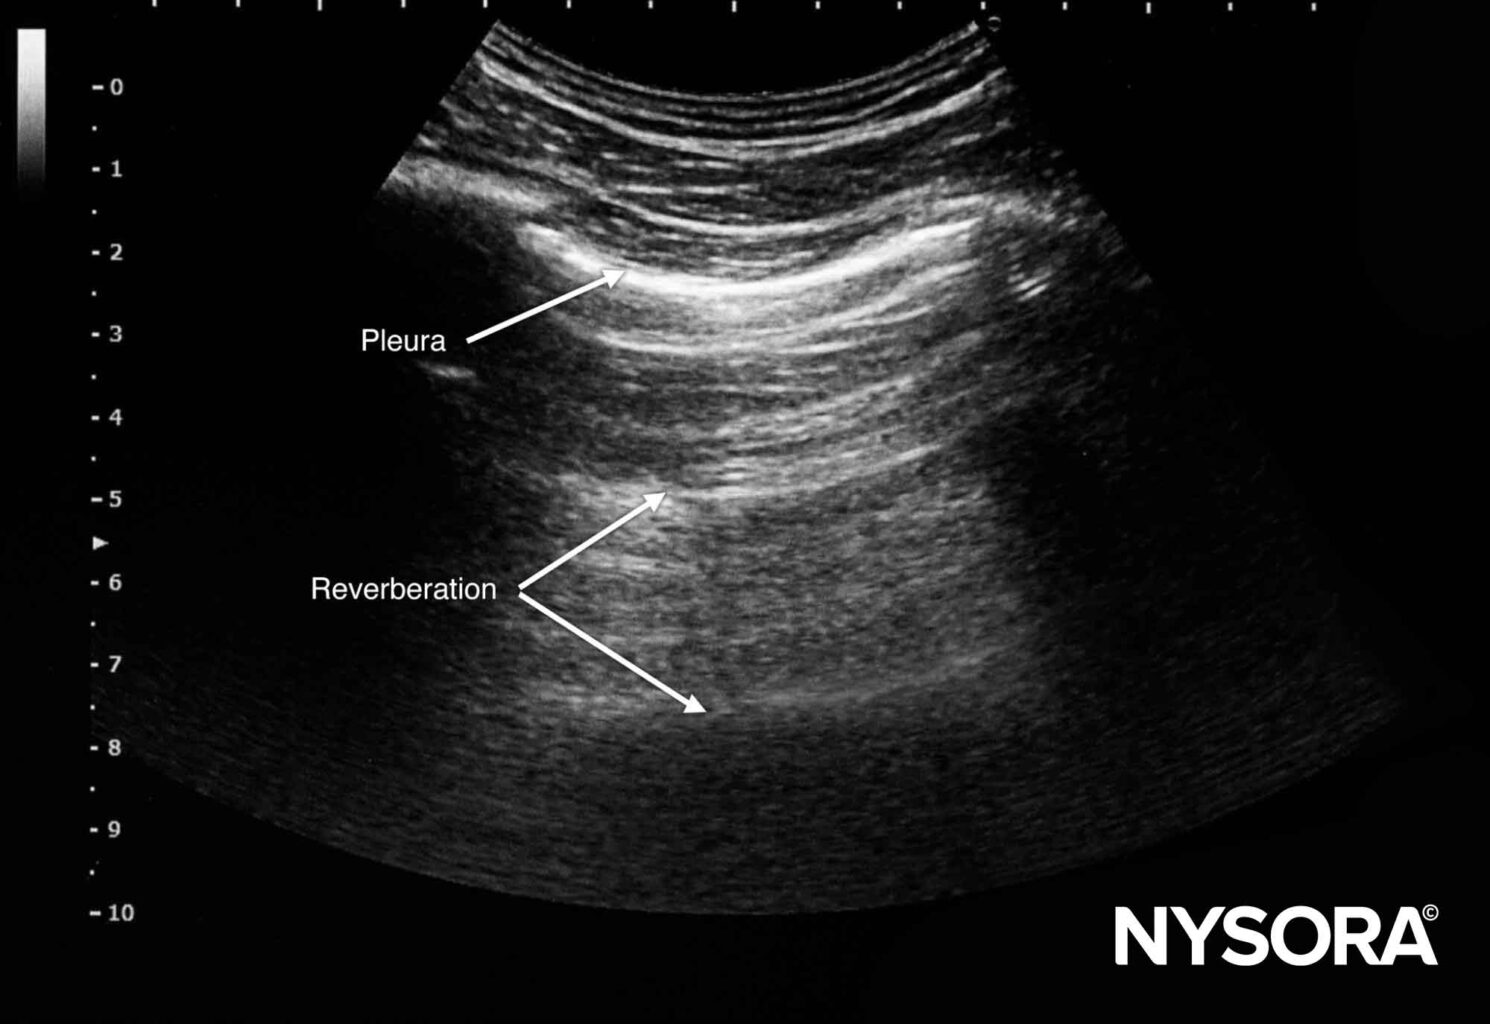
\includegraphics[width=6.5cm]{acoustic_reverberation}
  \caption{Acoustic reverberation artefact in ultrasound
    \cite{NysoraArtifacts}.\label{fig:acoustic_reverberation}}
\end{figure}

\section*{}
\subsection{Speckle}
\begin{itemize}
\item \popup{Speckle artifacts}{Also known by speckle noise.} are
  caused by the interference of sound waves with the echoes, resulting
  in a granular or \popup{speckled appearance of the image}{These
    artifacts can make it difficult to distinguish between small
    structures, such as blood vessels.}  \cite{NysoraArtifacts} (see
  Figure~\ref{fig:acoustic_speckle}).
\end{itemize}
\vspace{-2ex}
\begin{figure}[!h]
  \centering
  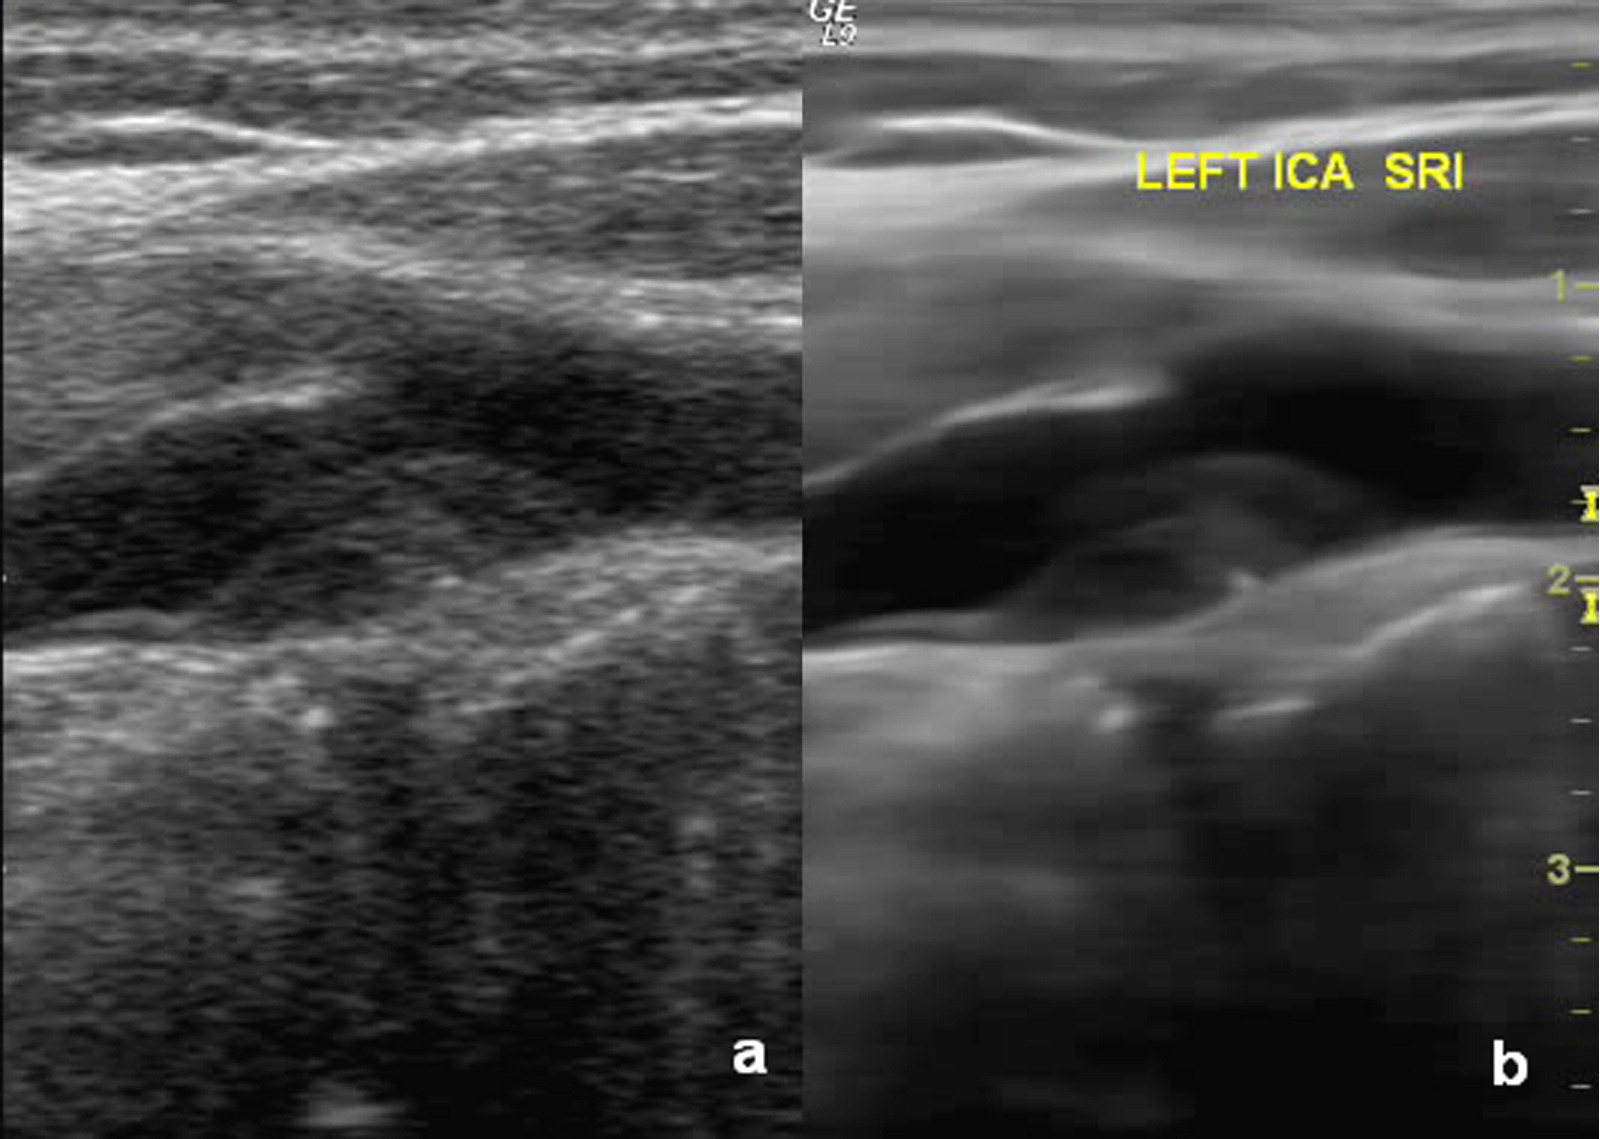
\includegraphics[width=6.5cm]{acoustic_speckle}
  \caption{Speckle noise in ultrasound
    \cite{LIASIS2008427}.\label{fig:acoustic_speckle}}
\end{figure}

\section*{}
\begin{itemize}
\item Speckle is usually modeled as \popup{multiplicative
    noise}{Multiplicative noise is proportional to the intensity of
    the clean signal.}. Its amplitude (which depends on the clean
  signal) follows a
  \href{https://en.wikipedia.org/wiki/Rayleigh_distribution}{Rayleigh
    distribution}, and its phase is
  \href{https://en.wikipedia.org/wiki/Discrete_uniform_distribution}{uniformly
    distributed}.

\item If multiple images are taken (changing the angle and
  orientation) and averaged \emph{spatial compounding}, speckle noise
  dimishes following a
  \href{https://en.wikipedia.org/wiki/Gamma_distribution}{Gamma
    distribution} \cite{bushberg2011essential}.
\end{itemize}


\section{Radiography}
\chapter{Radiography}
\vspace{-47ex}\hspace{38ex}
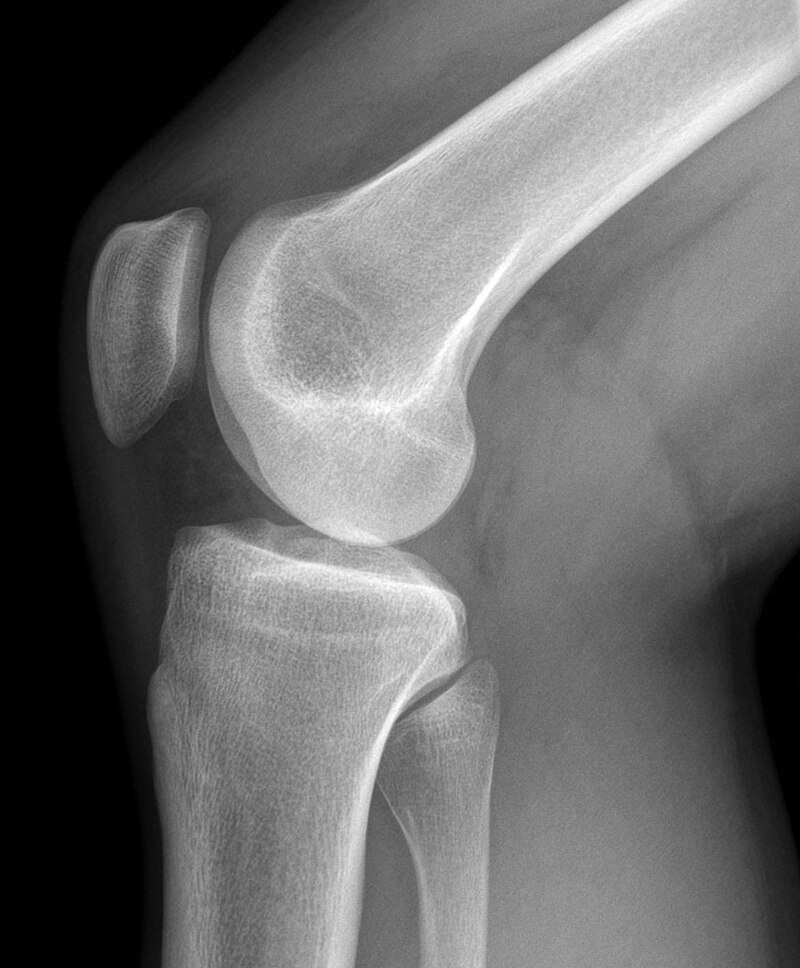
\includegraphics[width=10cm]{Knie-roentgen-r-seite} % https://upload.wikimedia.org/wikipedia/commons/thumb/8/89/Knie-roentgen-r-seite.jpg/800px-Knie-roentgen-r-seite.jpg

\section{X-ray and radiography}
\begin{itemize}
\item Radiography (X-ray 2D \popup{projection}{Radiography is also a
    projection imaging modality, meaning that each point on the image
    corresponds to information along a straight line through the
    patient}) is a transmission imaging modality where X-rays are
  emitted from a \popup{source}{An X-rays generator.}, pass through
  the patient, and are detected on the other side using a flat
  (usually \popup{digital TFT}{In digital X-ray detectors, a TFT array
    is used to read out electrical charges generated by the impact of
    the X-rays.}) detector (see
  Fig.~\ref{fig:projectional_radiography}).
\end{itemize}
\vspace{-4ex}
\begin{figure}[!h]
  \centering
  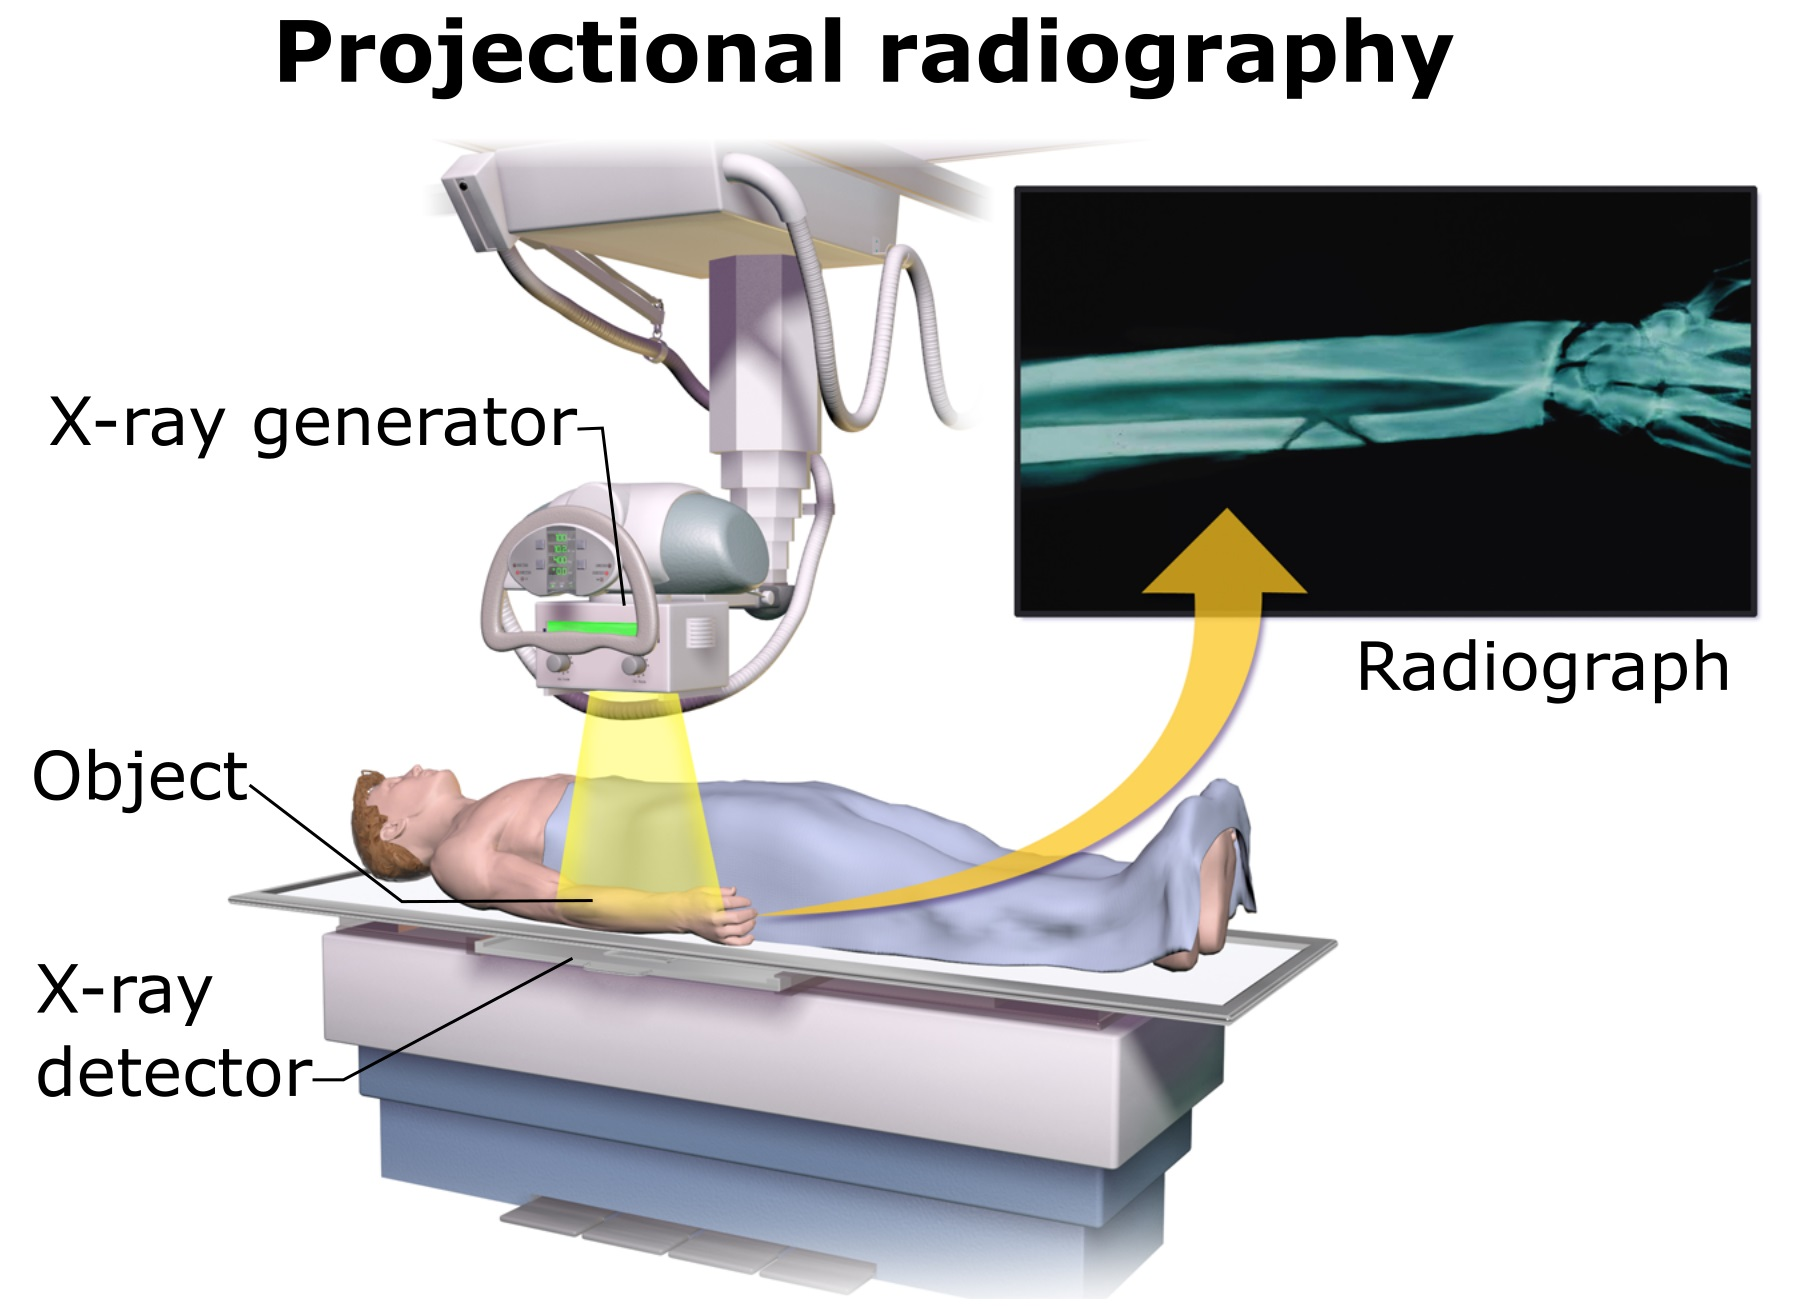
\includegraphics[width=6cm]{Projectional_radiography_components}
  \caption{Acquisition of projectional radiography, with an X-ray generator and a detector
    \cite{Wikipedia_X-ray_machine}.\label{fig:projectional_radiography}}
\end{figure}

\section{Transmission and attenuation}
\begin{itemize}
\item The X-ray attenuation of different tissues (e.g., bone, soft
  tissue, air) modify the homogeneous distribution of X-rays that
  enters the patient X-ray, forming the image in the detector
  \cite{bushberg2011essential} (see
  Fig.~\ref{fig:Attenuation-of-X-rays}).
\end{itemize}
\vspace{-3ex}
\begin{figure}[!h]
  \centering
  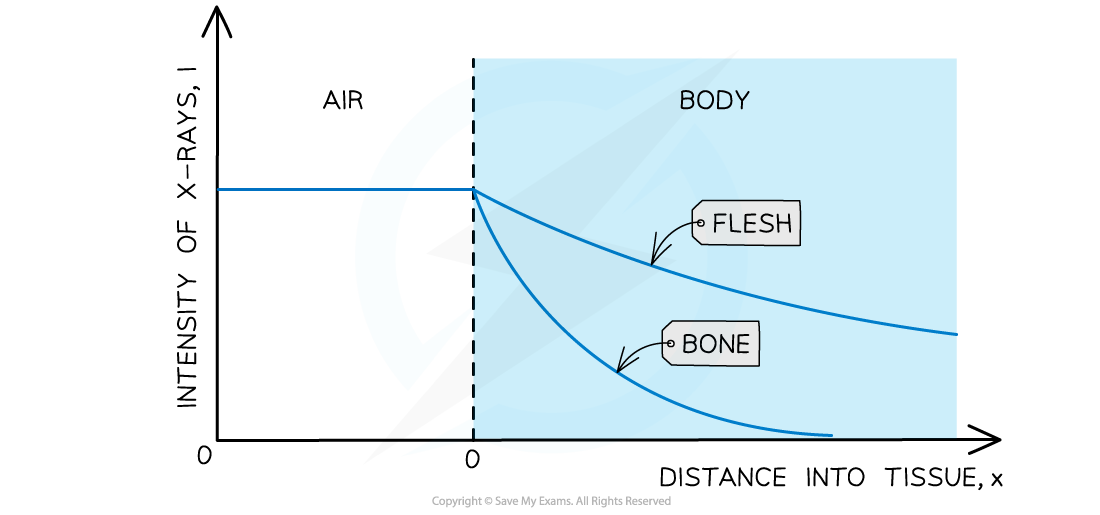
\includegraphics[width=9cm]{Attenuation-of-X-rays}
  \caption{Intensity-distance graph of X-rays for air and body
    \cite{Attenuation_X-rays}.\label{fig:Attenuation-of-X-rays}}
\end{figure}

\section{\glsentrylong{LAC} (\glsentryshort{LAC})}
\begin{itemize}
\item The X-rays are
  exponentially attenuated when they travel across the tissues \cite{wikipedia_LAC}.
\item To simplify numerical analysis and processing, we don't work
  directly with the attenuation coefficients but with the \glspl{LAC}, which
  are obtained applitying a logarithm operation.
\item For example, the numerical values used in
  Section~\ref{sec:FBP_example} are the result of computing the
  logarithm of the \popup{measured}{Returned by the detector.}
  attenuation coefficients.
\end{itemize}

\section{Why are we ``transparent''?}
\begin{itemize}
\item The \popup{fast ondulatory movement of X-ray-photons}{From 30
    petahertz (PHz)}{3x10$^{16}$ Hz.} to \popup{30 exahertz
    (EHz)}{3x10$^{19}$ Hz} makes them capable of \popup{penetrating
    soft tissues}{The higher the frequency of the X-rays photons, the
    higher their energy and the higher their penetration capability.}.
\end{itemize}
\vspace{-4ex}
\begin{figure}[!h]
  \centering
  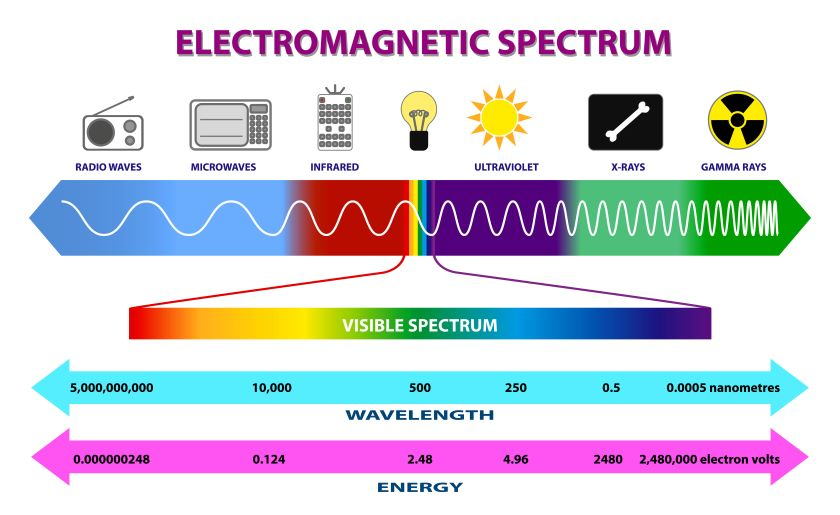
\includegraphics[width=8cm]{electromagnetic-spectrum}
  \caption{The electromagnetic spectrum
    \cite{X-rays_in_spectrum}.\label{fig:X-rays_in_spectrum}}
\end{figure}

\section{Ionization and biologic damage}
\begin{itemize}
\item X-rays are a form of \popup{ionizing radiation}{An ionizing
    radiation is capable of removing electrons from atoms or
    molecules, a process known as ionization (when an atom or molecule
    loses or gains electrons, it acquires a net electrical charge and
    becomes an ion).} (see Fig.~\ref{fig:ionization}), creating
  \popup{free radicals}{A free radical is an atom or molecule that has
    an unpaired electron in its outer shell. Because electrons prefer
    to exist in pairs, this unpaired electron makes the free radical
    highly unstable and very reactive.}.
\end{itemize}
\vspace{-3ex}
\begin{figure}[!h]
  \centering
  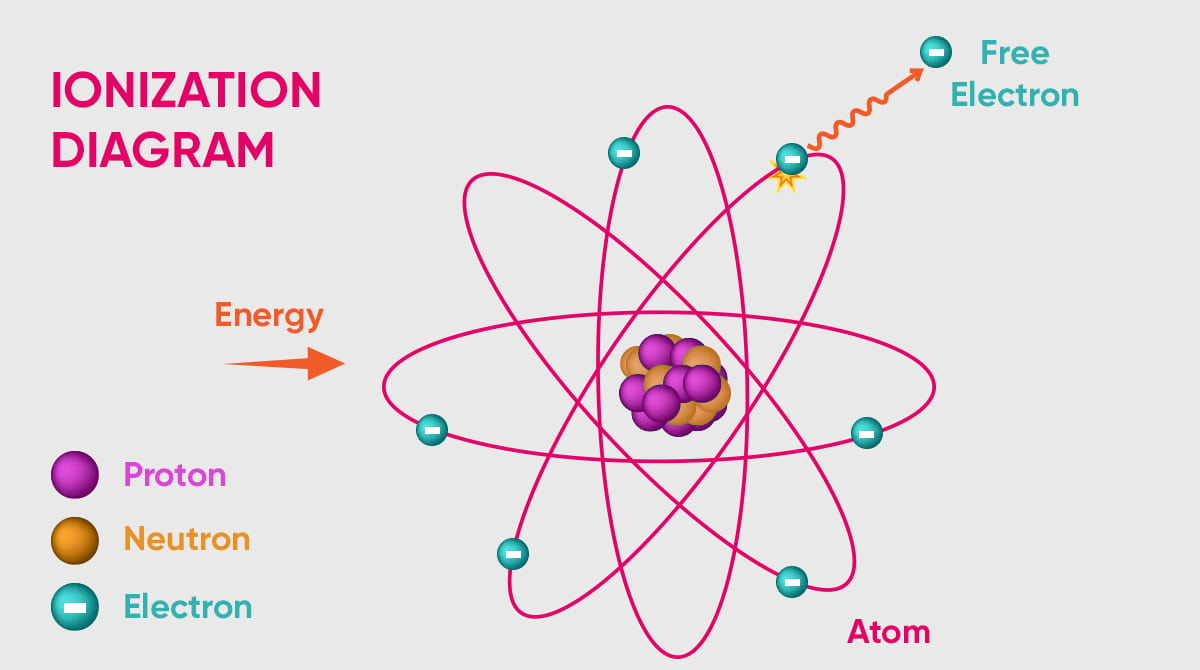
\includegraphics[width=8cm]{ionization-diagram}
  \caption{Ionization
    \cite{Perakende_ionization}.\label{fig:ionization}}
\end{figure}

\begin{itemize}
\item Free radicals are extremely reactive and can interact with
  biomolecules. This can produce a list of effects
  \cite{bushberg2011essential}:
  \begin{enumerate}
  \item \textbf{Short-term effects} (usually under high doses):
    \href{https://en.wikipedia.org/wiki/Radiation_burn}{burns},
    sickness.
  \item \textbf{Long-term effects}:Damage to DNA, could suffer
    \popup{mutations}{Although heavily irradiated cells often die
      during mitosis, preventing the propagation of seriously
      defective cells, damage to DNA at locations responsible for
      controlling cell division (e.g., oncogenes or tumour suppressor
      genes) could potentially lead to the formation of a tumour or
      cancer}, and \popup{tissue disfunction}{If there is ellular
      dysfunction, tissues can lose function and finally generate
      organ failure.}.
  \end{enumerate}
\end{itemize}

\section{Artifacts}
\begin{itemize}
\item In radiology, artifacts come from hardware failure, operator
  error (including the interaction/control with/of the patient) and
  software (post-processing) artifacts.
\item Only in digital radiology.
\end{itemize}

\section*{}
\subsection{Motion blur}
\vspace{-4ex}
\begin{figure}[!h]
  \centering
  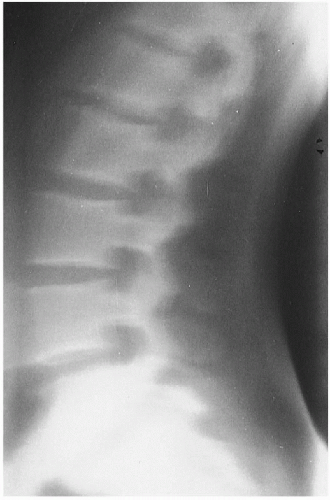
\includegraphics[width=3.5cm]{motion_blur_2}
  \caption{The image unsharpness was caused by patient movement
    \cite{radiology_key}.\label{fig:motion_blur}}
\end{figure}

\section*{}
\subsection{Static electricity}
\vspace{-3ex}
\begin{figure}[!h]
  \centering
  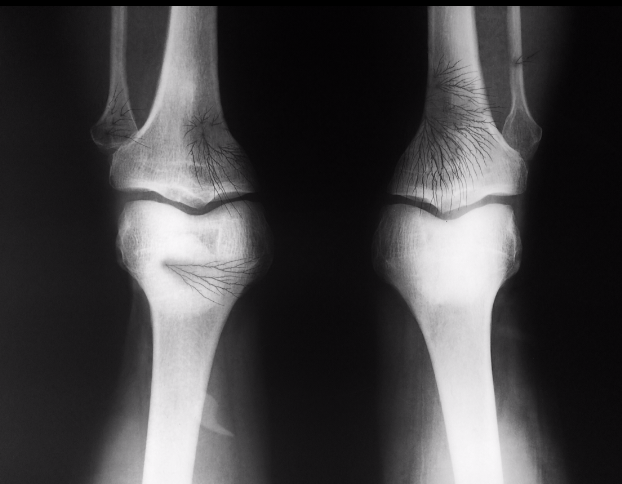
\includegraphics[width=7cm]{static-electricity}
  \caption{\cite{radiopaedia}.\label{fig:static_electricity}}
\end{figure}

\section*{}
\subsection{Dead pixel}
\vspace{-3ex}
\begin{figure}[!h]
  \centering
  \begin{tabular}{cc}
    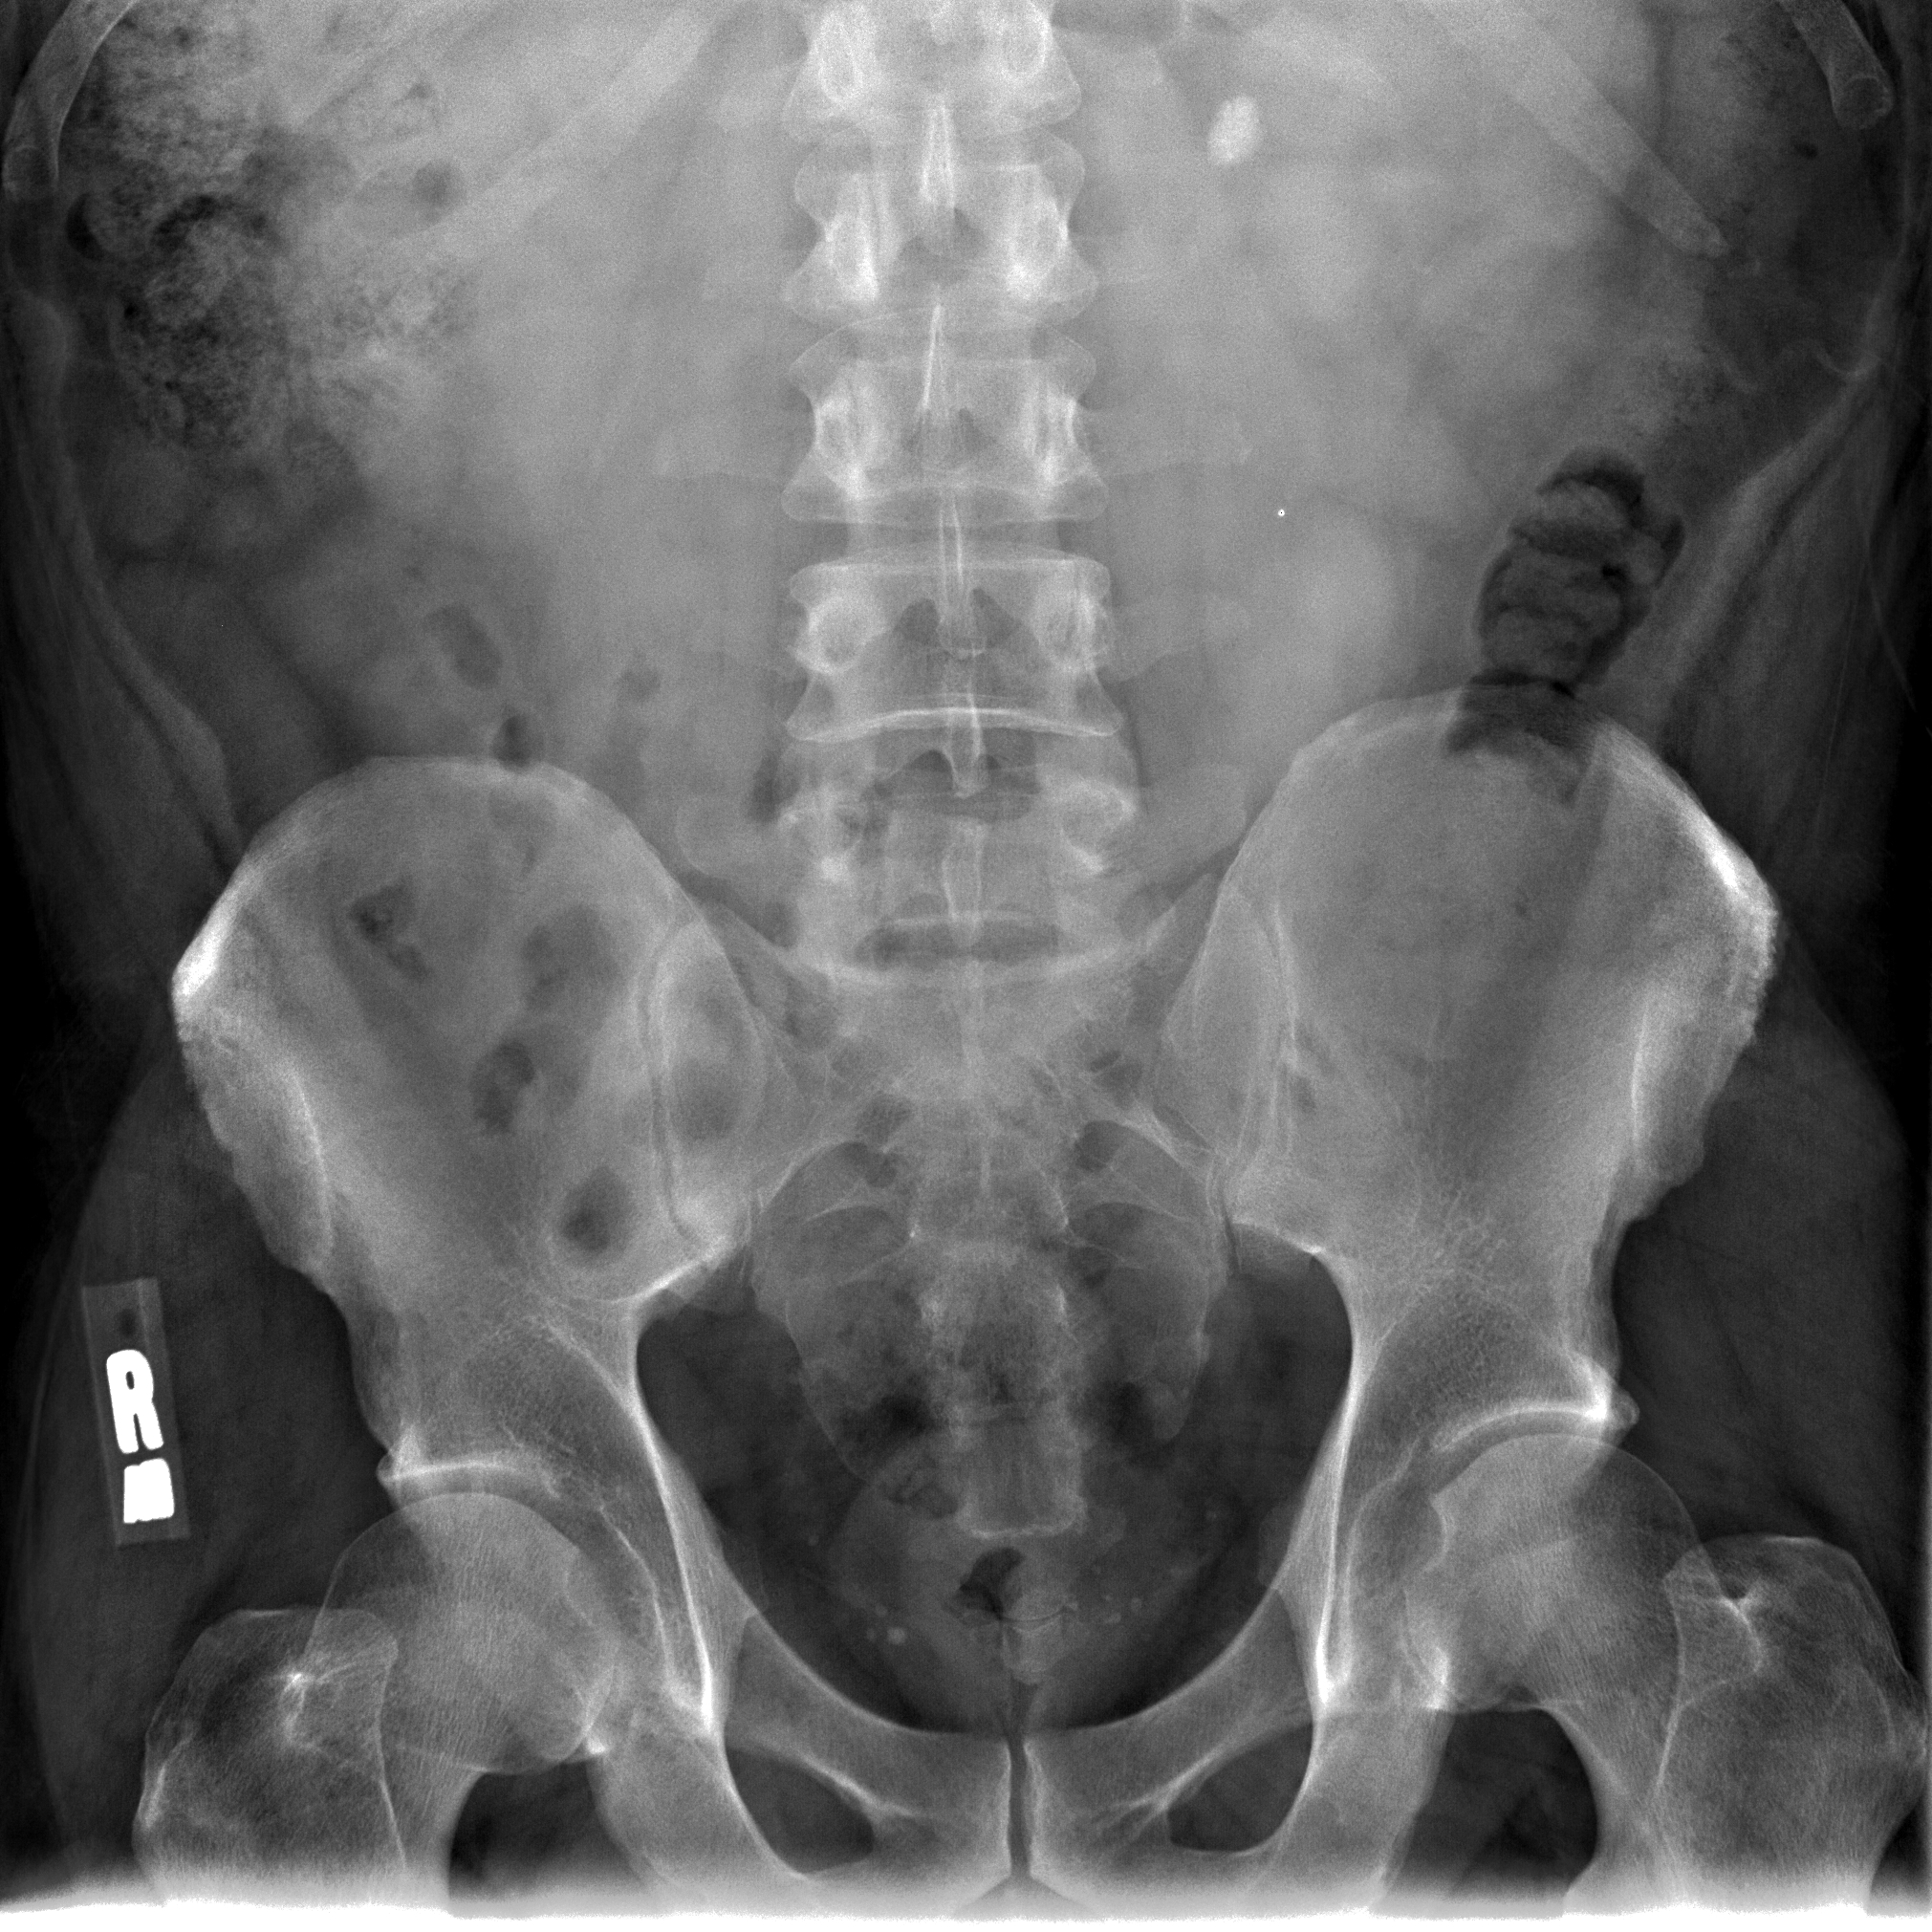
\includegraphics[width=5cm]{dead-pixel-artifact_frontal} &
                                                               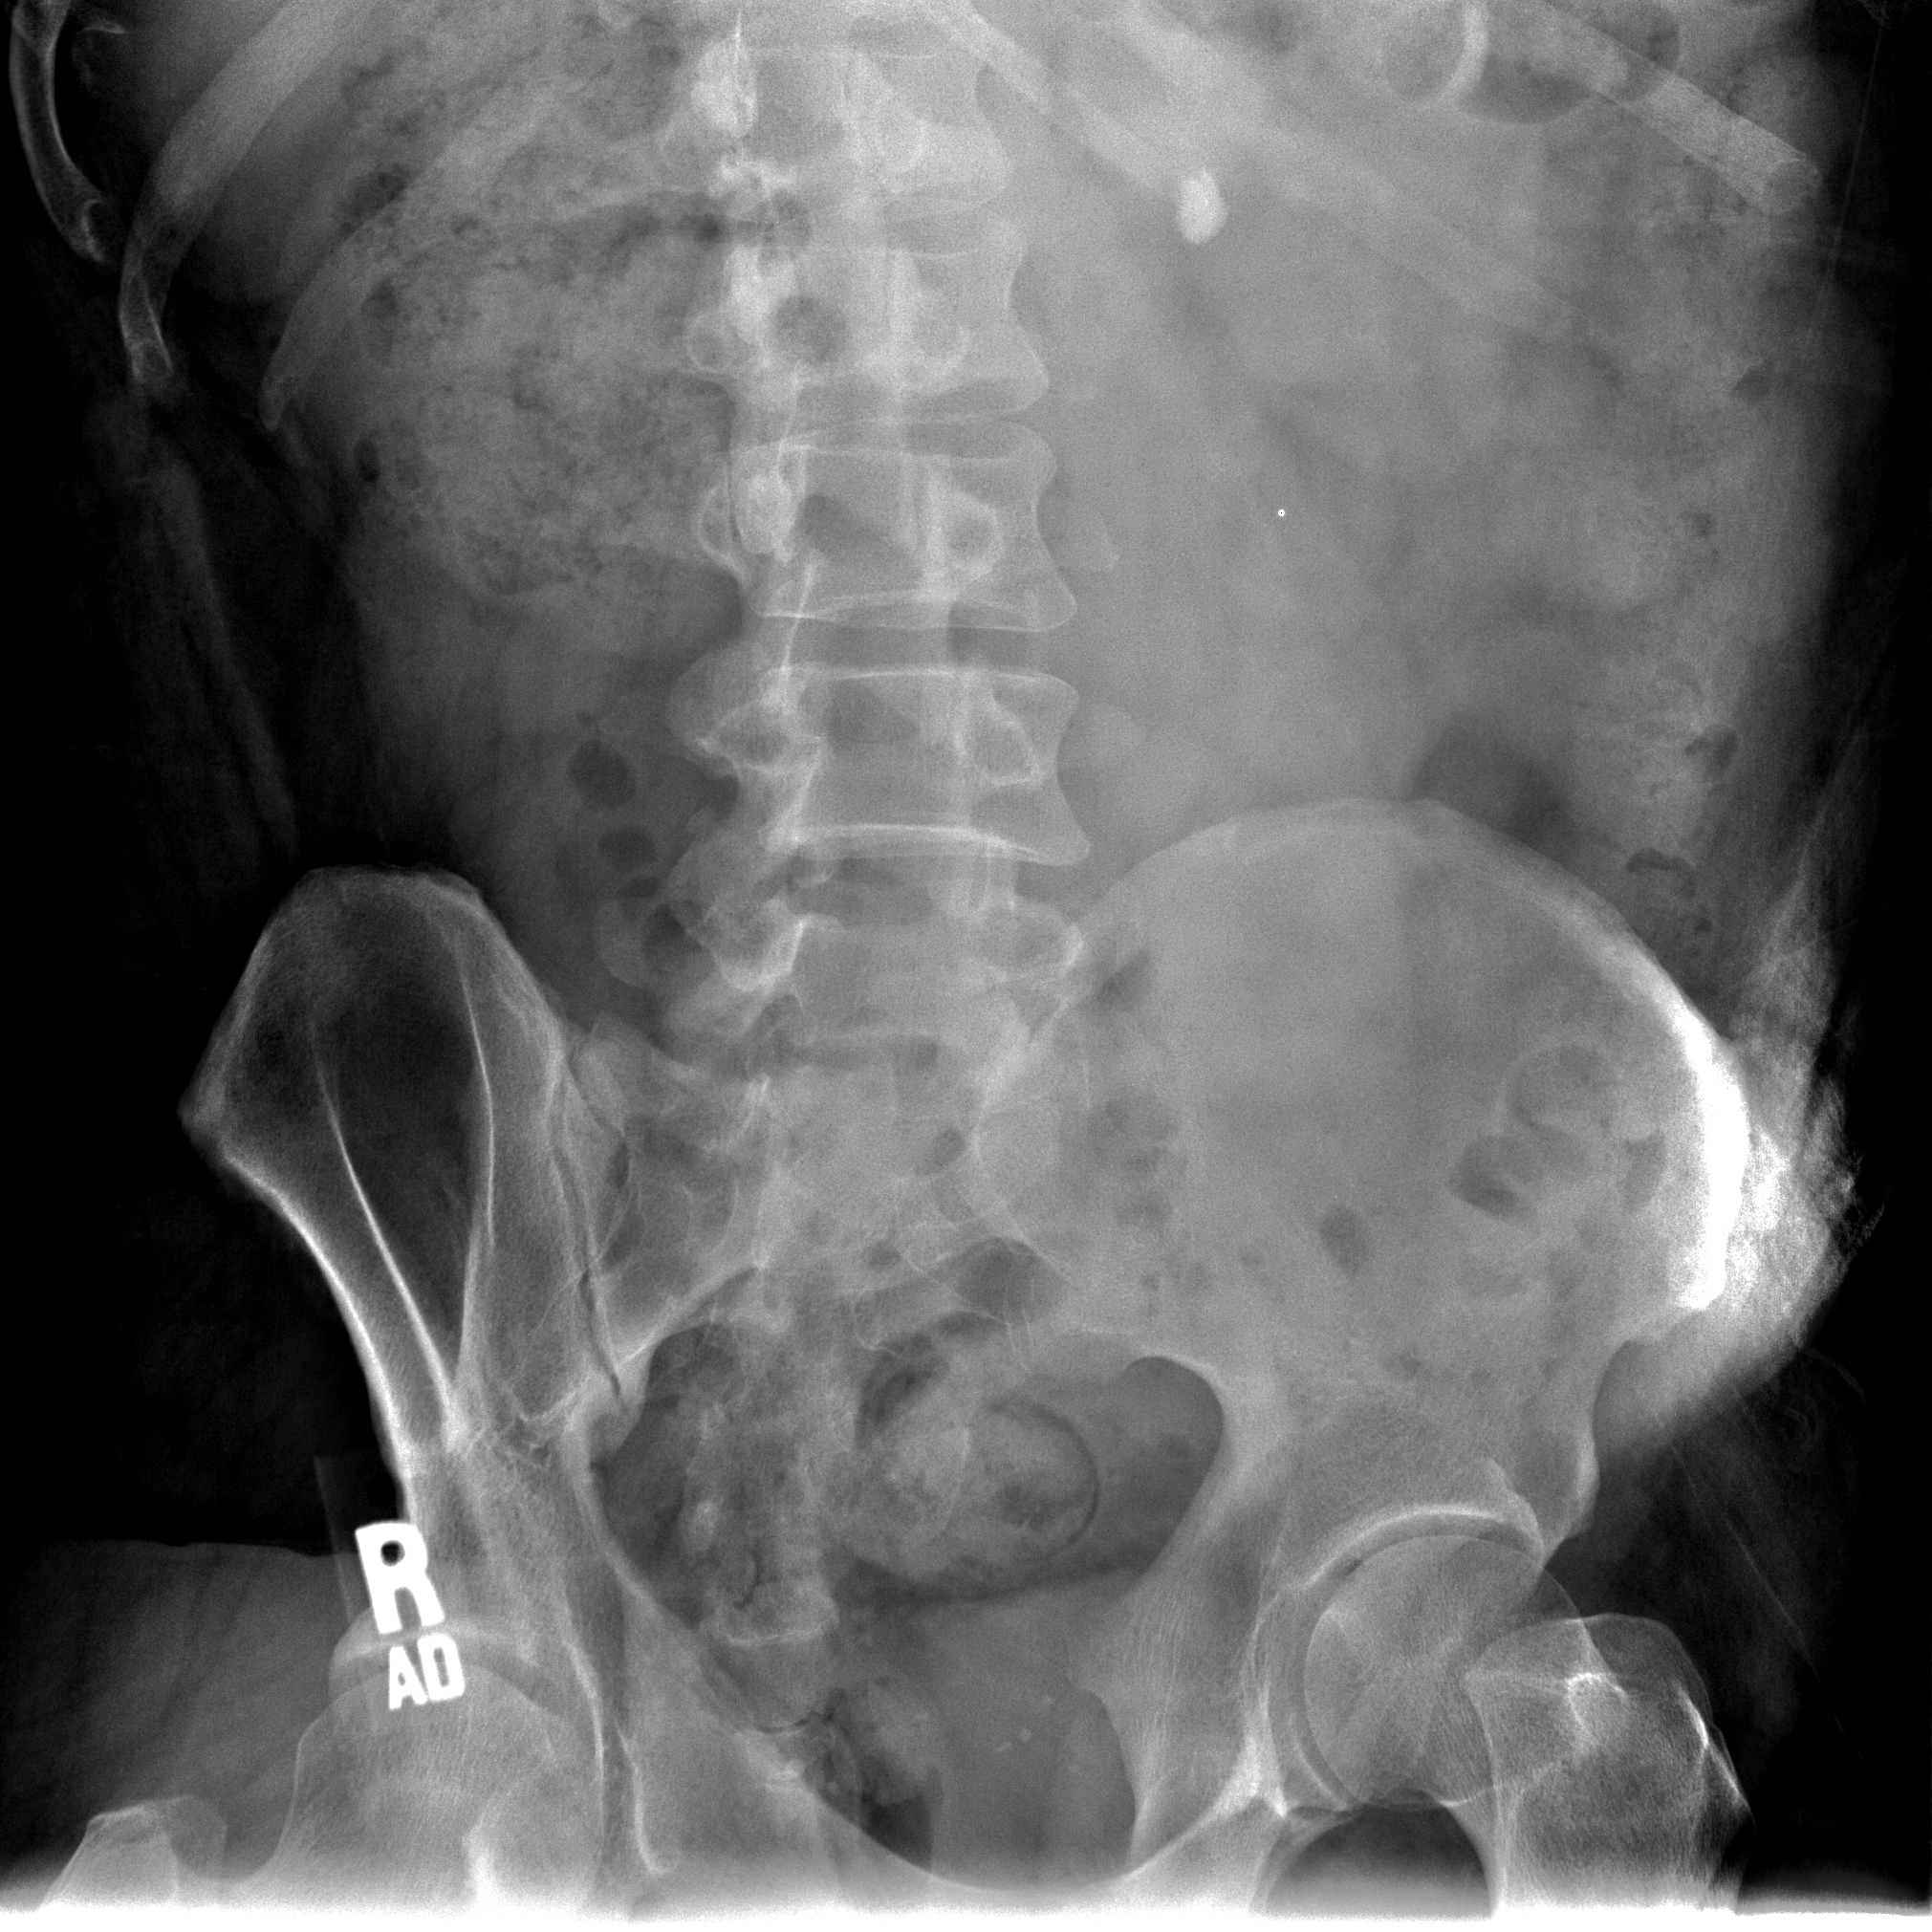
\includegraphics[width=5cm]{dead-pixel-artifact_oblique}
  \end{tabular}                                                
  \caption{Dead pixels are always white. \cite{radiopaedia}.\label{fig:dead_pixel}}
\end{figure}

\section*{}
\subsection{Under- and over-exposure}
\begin{itemize}
\item In digital radiology (down), the detector always generates a good contrast.
\item The main drawback is that, under-exposure usually have more noise.
\end{itemize}
\vspace{-4ex}
\begin{figure}[!h]
  \centering
    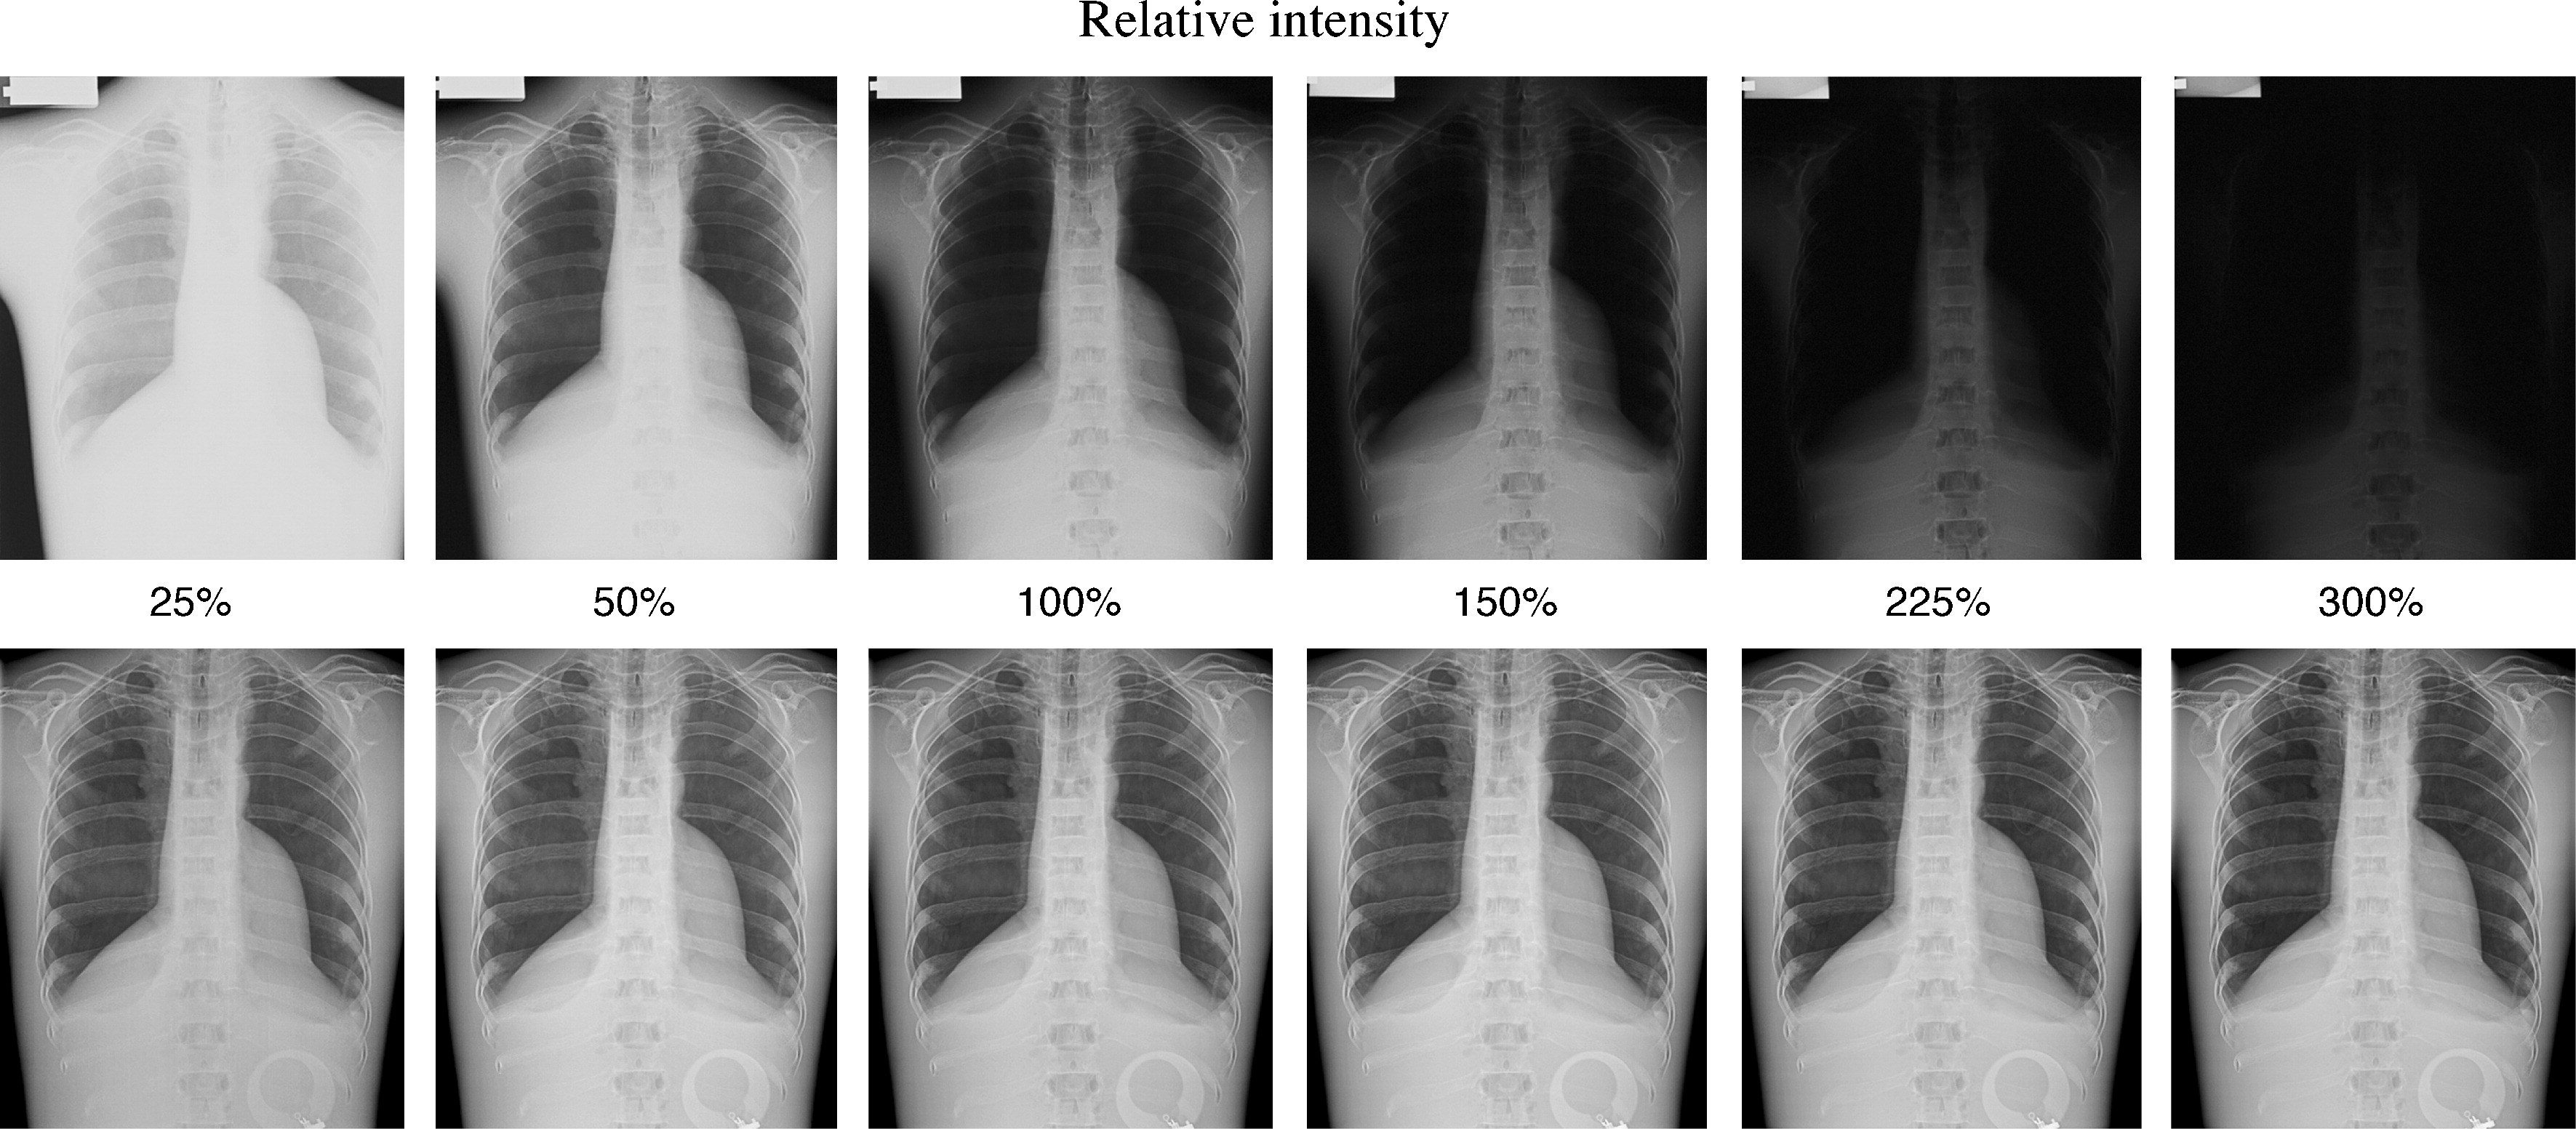
\includegraphics[width=9cm]{X-ray_exposure}
    \caption{Exposure impact (up: analog, down: digital)
      \cite{VELDKAMP2009209}.\label{fig:exposure}}
\end{figure}

\section{Mammography}
\begin{itemize}
\item Mammography is the 2D X-rays projection\\ of the breast
  \cite{bushberg2011essential}.
\item Makes use of much lower x-ray energies\\ than general purpose
  radiography.
\end{itemize}
\vspace{-20ex}
\begin{figure}[!h]
  \begin{flushright}
    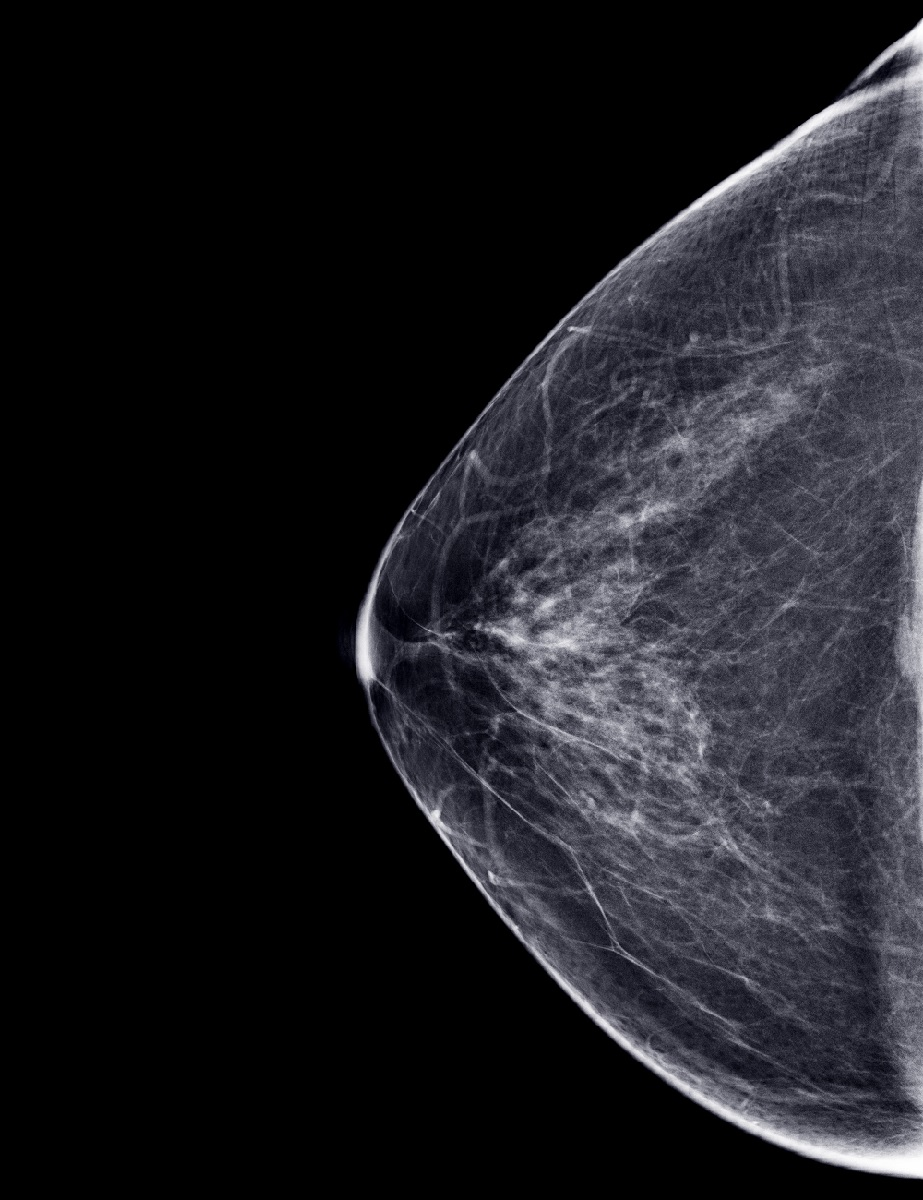
\includegraphics[width=4.5cm]{normal_mammogram}
    \end{flushright}
    \caption{Mamogram \cite{CDC_mammograms}.\label{fig:mamogram}}
\end{figure}

\section{Fluoroscopy}
\begin{itemize}
\item A fluoroscope produces real-time X-ray images with high temporal
  resolution (e.g., 30 frames per second), allowing continuous motion
  viewing, useful for \popup{interventional procedures}{Fluoroscopy is
    used for positioning catheters in arteries, visualizing contrast
    agents in the \gls{GI} tract, and for other medical applications
    such as invasive therapeutic proce- dures where real-time image
    feedback is necessary. It is also used to make x-ray movies of
    anatomic motion, such as of the heart or the esophagus.}
  \cite{bushberg2011essential}.
\item Compared to ``one-shot'' radiography, the images are more noisy.
\item
  \href{https://en.wikipedia.org/wiki/Fluoroscopy#/media/File:Normal_barium_swallow_animation.gif}{Swallowing
    of varium} \cite{Wikipedia_Fluoroscopy}.
\end{itemize}

\section{Quantum noise}
\begin{itemize}
\item Quantum noise is the most common noise in X-rays imaging.
\item It is directly related to photon counting (fewer photons
  $\rightarrow$ more noise).
\item More evident (lower \gls{SNR}) at low radiation doses.
\end{itemize}
\vspace{-4ex}
\begin{figure}[!h]
  \centering
    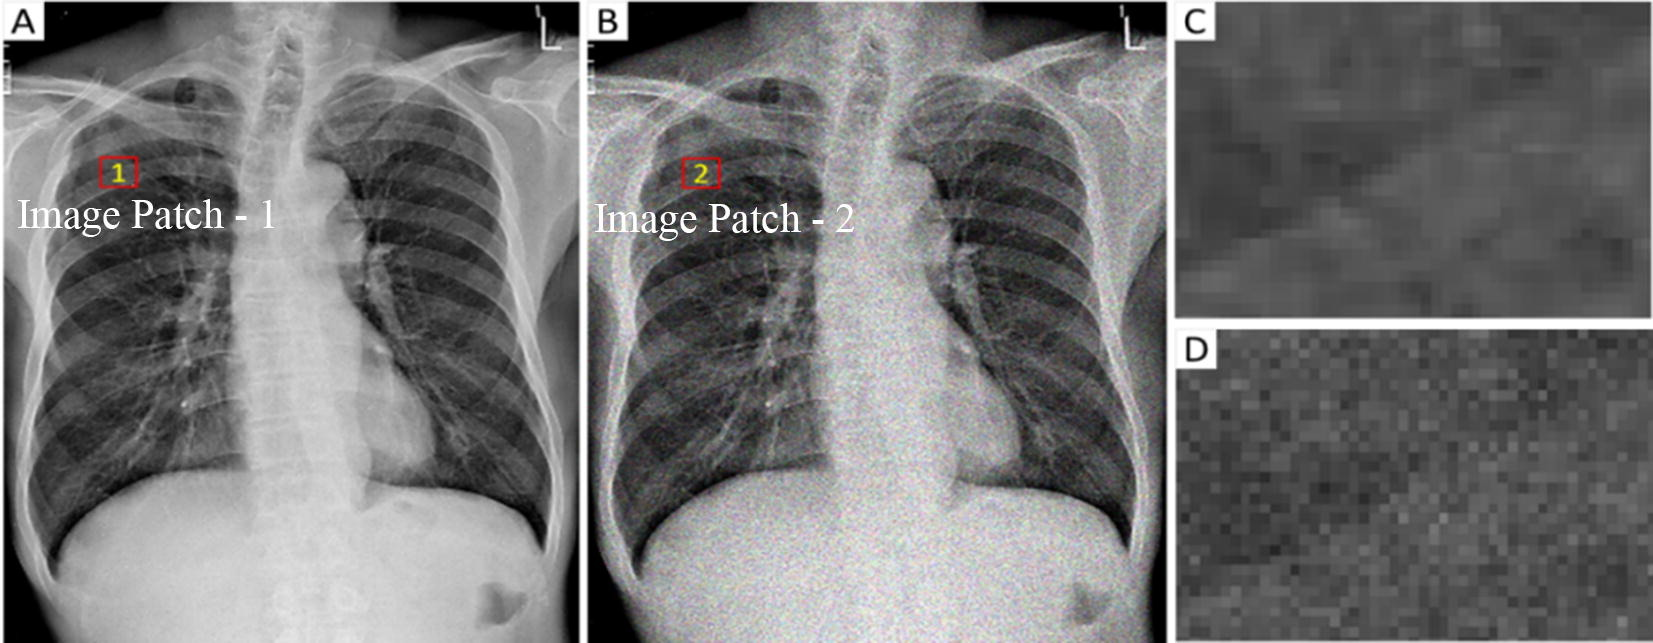
\includegraphics[width=10cm]{quantum_noise_X-rays}
    \caption{Quantum noise in radiology
      \cite{CHANDRA2020107426}.\label{fig:quantum_noise_X-rays}}
\end{figure}

\label{sec:radiography_quantum_noise}
\begin{itemize}
\item The amplitude of quantum noise depends on the (clean) signal amplitude.  
\item On average, quantum noise appears on all the frequencies and is typically \href{https://en.wikipedia.org/wiki/Colors_of_noise}{colored}.
\end{itemize}
\vspace{-4ex}
\begin{figure}[!b]
  \centering
    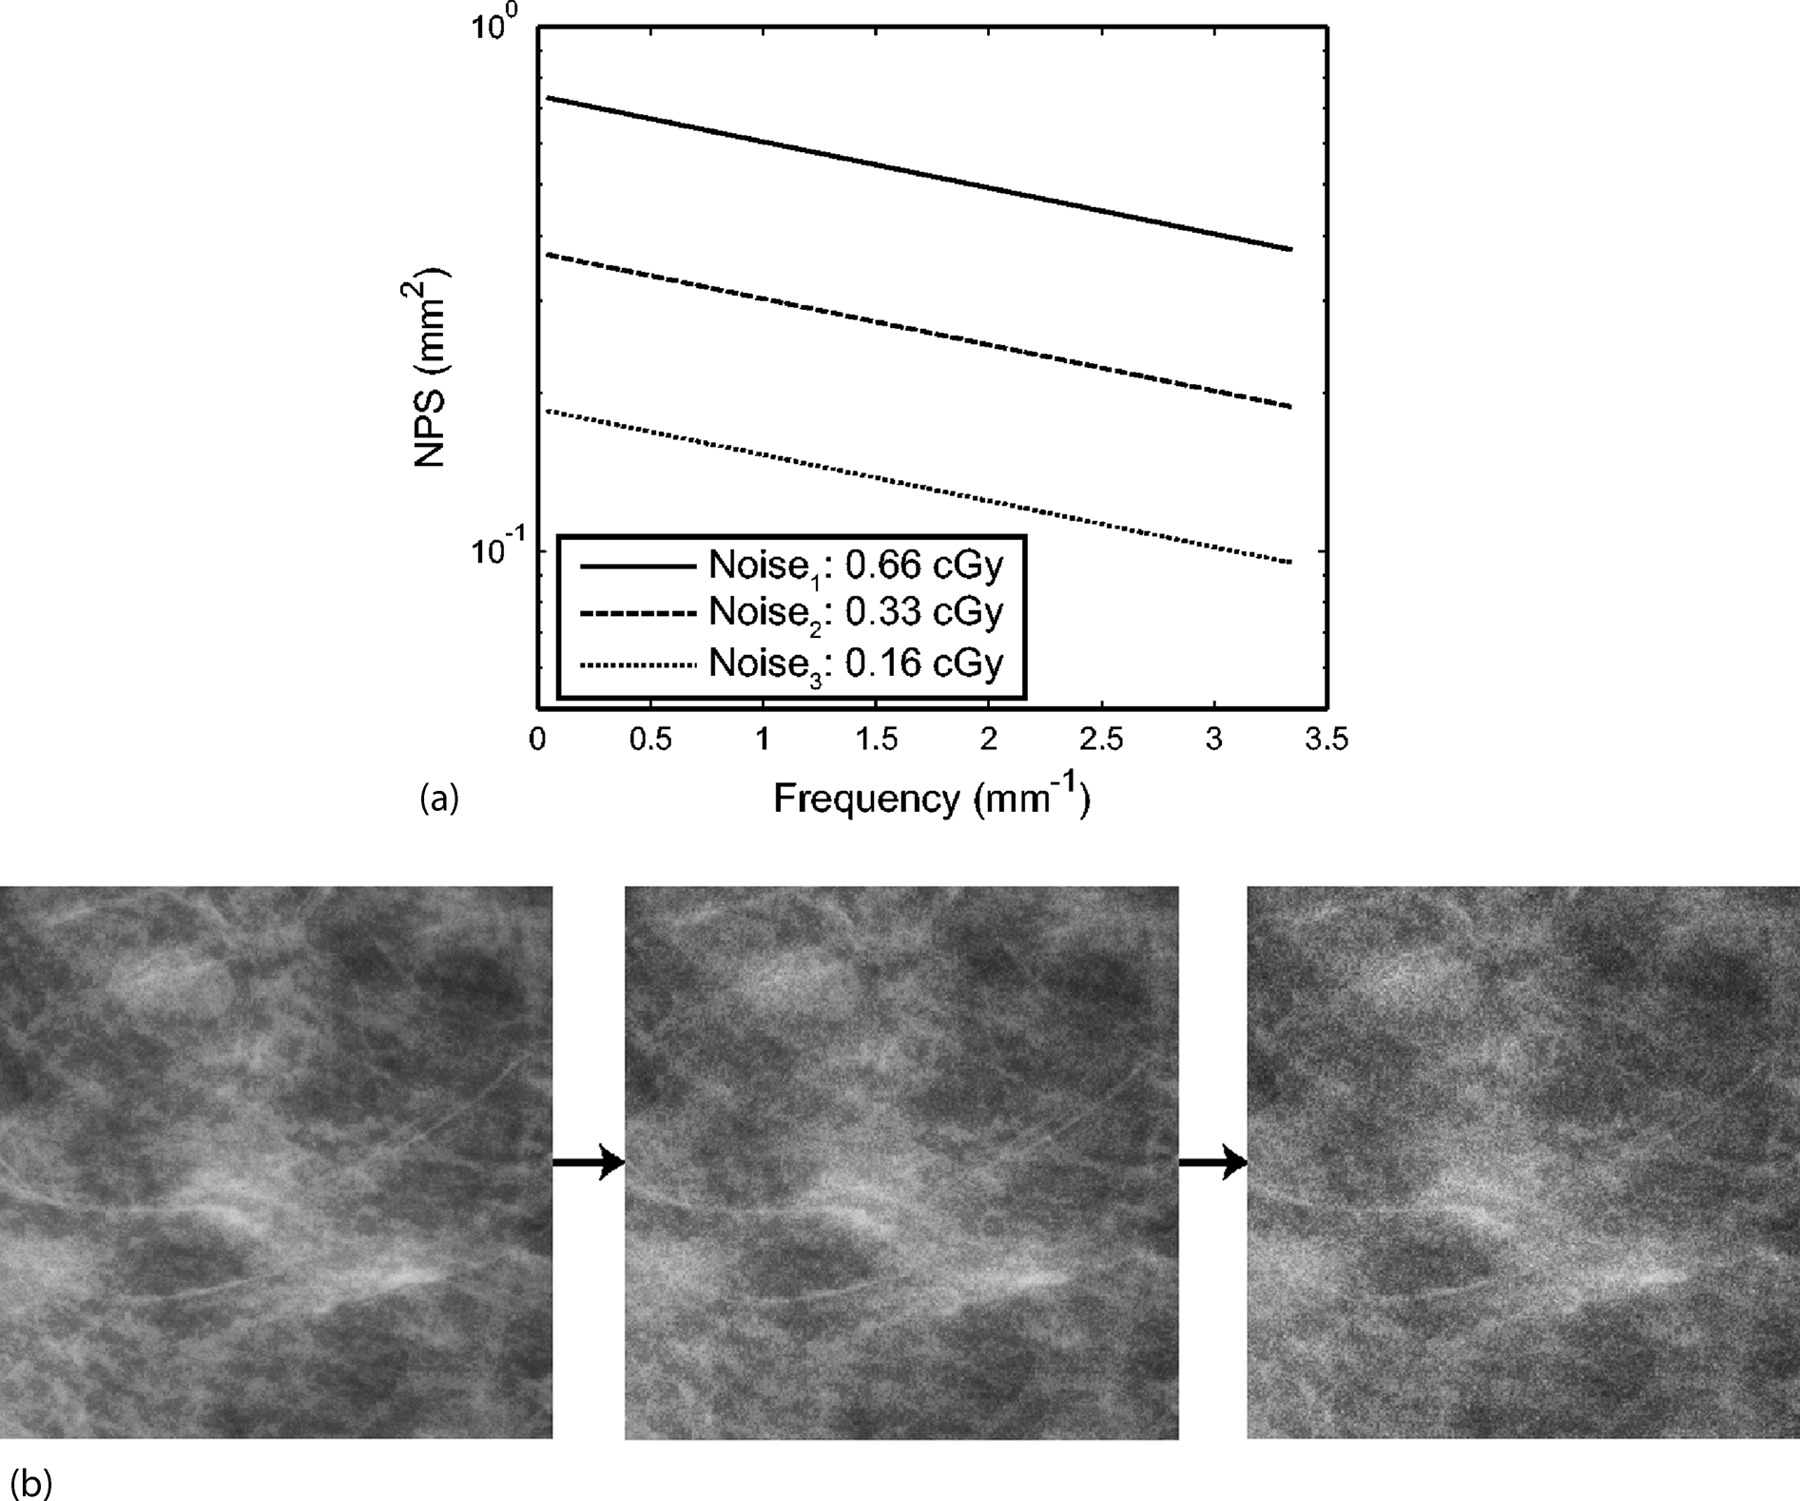
\includegraphics[width=6cm]{quantum_noise_mammography}
    \caption{Average quantum noise spectrum (up), some examples in mammograms (below) 
      \cite{saunders2007does}.\label{fig:quantum_noise_X-rays_spectrum}}
\end{figure}


\section{Mamography}
\input{mamography}

\section{Fluoroscopy}
\chapter{Fluoroscopy}

Produces real-time X-ray images with high temporal resolution (e.g.,
30 frames per second) but at a low dose (and therefore low \gls{SNR})
per image compared to radiography. This allows for continuous motion
viewing, useful for interventional procedures.\footnote{Fluoroscopy is
  used for positioning catheters in arteries, visualizing contrast
  agents in the \gls{GI} tract, and for other medical applications
  such as invasive therapeutic proce- dures where real-time image
  feedback is necessary. It is also used to make x-ray movies of
  anatomic motion, such as of the heart or the esophagus
  \cite{bushberg2011essential}.}

When possible, frame averaging is used to increase the
SNR.\footnote{Fluoroscopy systems provide excellent temporal
  resolution, a feature that is the basis of their clinical
  utility. However, fluoroscopy images are also relatively noisy, and
  under certain circumstances it is appropriate and beneficial to
  (reduce) temporal resolution for lower quantum noise. This can be
  accomplished by averaging a series of images. Appreciable frame
  averaging can cause notice-able image lag with reduced temporal
  resolution. The compromise depends on the specific fluoroscopic
  application and the preferences of the user
  \cite{bushberg2011essential}.}


\section{Computed Tomography (CT)}
\chapter{Computed Tomography (CT)}

CT images are produced by passing x-rays through the body at a large
number of angles, by rotating the x-ray tube around the body. A
detector array, opposite the x-ray source, collects the transmission
projection data. The numerous data points collected in this manner are
synthesized by a computer into tomographic images of the patient. The
term tomography refers to a picture (graph) of a slice (tomo). The
advantage of CT over radiography is its ability to display
three-dimensional (3D) slices of the anatomy of interest, eliminating
the superposition of anatomical structures and thereby presenting an
unobstructed view of detailed anatomy to the physician
\cite{bushberg2011essential}.

The CT volume data set is essentially isotropic, which has led to
the increased use of coronal and sagittal CT images, in addition to
traditional axial images in CT. There are a number of different
acquisition modes available on modern CT scanners, including
dual-energy imaging, organ perfusion imaging, and prospectively gated
cardiac CT. While CT is usually used for anatomic imaging, the use of
iodinated contrast injected intravenously allows the functional
assessment of various organs as well \cite{bushberg2011essential}.

Radon transform


\section{Resources}

\bibliography{tomography}


\section{Single Photon Emission Computed Tomography (SPECT)}
\chapter[\glsentrylong{SPECT} (\glsentryshort{SPECT})]{Single Photon Emission\\Computed Tomography (SPECT)}
\vspace{-45ex}
\begin{flushright}
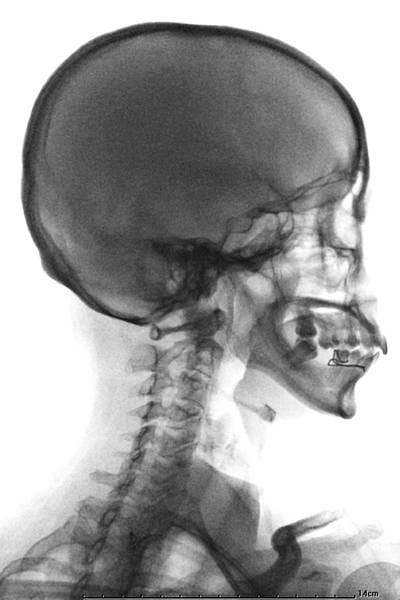
\includegraphics[width=4.5cm]{SPECT_example} % https://www.cidrad.com/wp-content/uploads/2024/06/testicular-ultrasound-riverside-county-ca-usa-near-me-400-600.jpg
\end{flushright}

\section{Acquisition}
\begin{itemize}
\item \gls{SPECT} is the tomographic counterpart of nuclear medicine
  planar imaging, just like CT is the tomographic counterpart of
  radiography \cite{bushberg2011essential,wikipedia_SPECT}.
  
\item In SPECT, a nuclear camera records X- or Gamma-ray emissions
  from the patient from a series of different angles around the
  patient.
  
\item  These projection data are used to reconstruct a series of
  tomographic emission images.

\item The spatial resolution of the images is inversely proportional
  to the distance between the patient and of the \popup{camera}{The
    camera uses a collimator to determine the direction of the
    photons. This generates a low detection efficiency because the
    collimator filters out over 99.9\% of the emitted photons. The
    design of the collimator inherently compromises between spatial
    resolution and detection efficiency}.
\end{itemize}

\section{Clinical applications}
\begin{itemize}
\item SPECT images provide diagnostic functional information similar
  to nuclear planar examinations (functional information about organ
  physiology) ; however, their tomographic nature allows physicians to
  better understand the precise distribution of the radioactive agent,
  and to make a better assessment of the function of specific organs
  or tissues within the body.
\item The same radioactive isotopes are used in both planar nuclear
  imaging and SPECT \cite{bushberg2011essential}.
\end{itemize}

\section{Image quality}
\begin{itemize}
\item The resolution is limited (hundres of pixels in each dimension)
  by two reasons:
  \begin{enumerate}
  \item The detection efficiency (which is very low) depends on the
    pixel-size.
  \item Each projection requires dozens of seconds
    \cite{abdulla2025SPECT}.
  \end{enumerate}
\item Althought it is based on the same imaging technology than PNI,
  it usually provided improved contrast and reduced structural noise
  by averaging counts from overlapping structures
\end{itemize}

\section{Positron Emission Tomography (PET)}
\chapter[\glsentrylong{PET} (\glsentryshort{PET})]{Positron Emission\\Tomography (PET)}
\vspace{-40ex}
\begin{flushright}
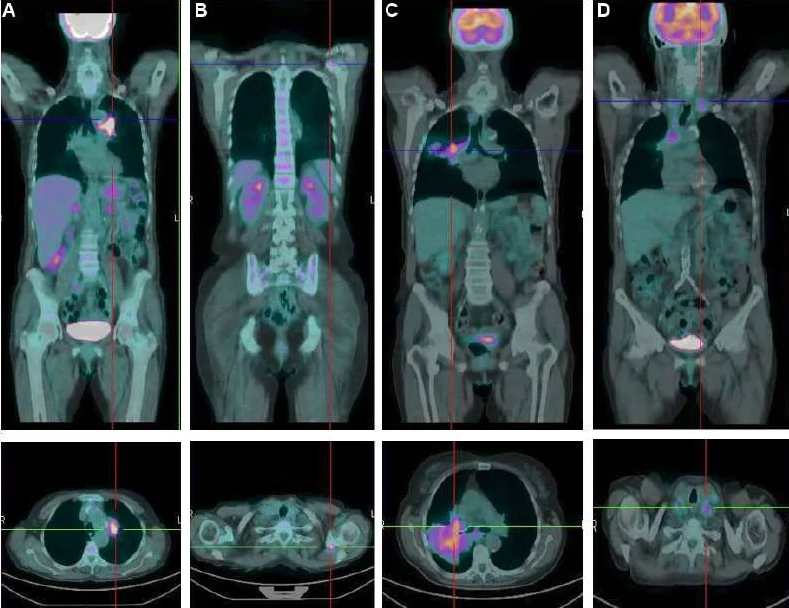
\includegraphics[width=6.5cm]{PET} % https://ksimg.com/wordpress/wp-content/uploads/2022/02/pet-ct.jpg
\end{flushright}

\section{Acquisition}
\begin{itemize}
\item Such as SPECT, PET is a tomographic nuclear imaging system
  \cite{abdulla2025PET,wikipedia_PET}.
\item Employs \popup{annihilation coincidence detection
    (ACD)}{Positron-emitting radioisotopes decay and release a
    positron. This positron travels a short distance, then annihilates
    with an electron from the surrounding tissue, converting their
    mass into two 511-keV photons. These two photons are emitted
    simultaneously and in nearly opposite directions (approximately
    180 degrees apart). PET scanners detect these coincident photon
    pairs using rings of detectors and specialised circuitry. ACD is
    significantly more efficient than collimation and avoids the
    degradation of spatial resolution with increasing distance from
    the detector.} instead of collimation to determine the procedence
  of the radiation that reach the detector.
\item Only uses \popup{positron-emitting radionuclides}{F-18
    fluorodeoxyglucose (FDG) is the most widely used PET
    radiopharmaceutical. Due to their generally short half-lives, PET
    radionuclides often require a cyclotron to be located nearby or
    on-site}.
\item PET scanners are more ``open'' than SPECT scanners because the
  resolution of the images is not so dependent on the distance of the
  camera to the patiend.
\item PET is \popup{more expensive}{A PET/CT system can cost
    approximately twice that of a SPECT/CT system} than SPECT.
\end{itemize}

\section{Clinical applications}
\begin{itemize}
\item As SPECT, it is mainly used to \popup{visualise physiological
    function}{The most common application of PET (especially with F-18
    FDG) is in oncology for differentiating malignant neoplasms,
    staging cancer, and monitoring treatment response.}
  \cite{bushberg2011essential}.
\end{itemize}

\section{Image quality}
\begin{itemize}
\item Compared to SPECT, PET has much higher count rate sensitivity
  and, generating less noise.
\item Therefore, PET images can be reconstructed with much higher
  spatial frequency \cite{abdulla2025NIQ}.
\end{itemize}


\chapter{Storage}
\part{Medical Images Storage}

\chapter{Basic concepts}

\section{Storage media charactaristics}
\begin{enumerate}
\item \textbf{Capacity}: This is the total amount of data that a
  storage medium can hold. It's typically measured in \popup{B}{byte}s
  (8 \popup{bits, where a bit represents a logical state with one of
    two possible values.}), \popup{KB}{kilobyte}s
  ($1\text{KB} = 2^{10}\text{B}$), \popup{MB}{megabytes}s
  ($1\text{MB} = 2^{10}\text{KB}$), \popup{GB}{gigabyte}s
  ($1\text{GB} = 2^{10}\text{MB}$), \popup{TB}{terabyte}s
  ($1\text{TB} = 2^{10}\text{GB}$), and \popup{PB}{petabyte}s
  ($1\text{PB} = 2^{10}\text{GB}$).
\item \textbf{Volatility}: If the media need to connected to a current supply (for example, the \gls{RAM} memory of a computer), the media is said \emph{volatile}.
\item \textbf{\gls{WORM}}: A \gls{CDROM}, for example.
\end{enumerate}
\begin{itemize}
\item There are many storage media capable of storing digital images (some allow
\begin{enumerate}
\item 
\item Common massive storage systems (not only used for medical images) are:
\begin{enumerate}
\item \textbf{Cloud Storage} (Google Drive, Microsoft One Drive,
etc.): data is stored in remote servers accessed over the Internet.
\item \textbf{NAS (Network-Attached Storage)}: data is stored in a
\popup{specialized computer}{The computer rarely has a keyboard or
monitor, and has many hard drive bays.} (connected to the
\popup{LAN}{Local Area Network.}) that usually mounts several disks
with some type of \popup{RAID}{Redundant Array of Independent Disks.}
configuration.
\end{enumerate}
\end{itemize}
\vspace{-4ex}
\begin{figure}[!b]
  \centering
  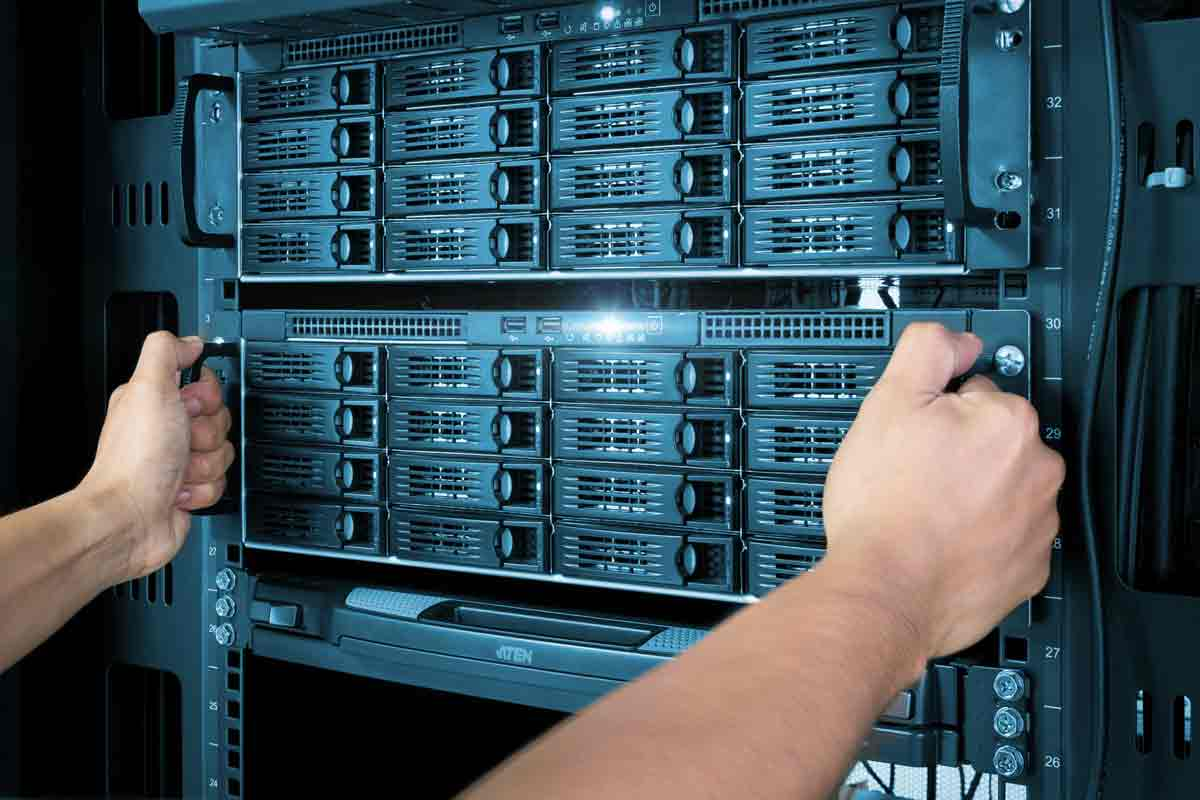
\includegraphics[height=3.5cm]{servidor-nas}
  \caption{A NAS \cite{AURUM_NAS}.\label{fig:NAS}}
\end{figure}

\section{Arrays of redundant disks}
\begin{itemize}
\item A \gls{RAID} is a logical disk that is able to work even when some of the \popup{physical disks}{That actually store the data.} fail. These are some of the existing configurations:
  \begin{enumerate}
  \item RAID-0 (Striping): \popup{No redundancy}{To maximize capacity,
      splits data across drives. This means that if a physical disk
      stops working, a loss of data will happen.}.
  \item RAID-1 (Mirroring): \popup{Maximum redundancy}{All physical
      disks contain the same data. To lost data all disks must fail at
      the same time.}.
  \item RAID-5 (Striping with Parity): \popup{One disk
      redundancy}{This configuration can only tolerate the failure of
      one disk.}. When the broken disk is replaced, the RAID must rebuild the parity information. During this time, no other disk can fail.
  \item RAID-6 (Double Parity): \popup{Two disks
      redundancy}{Tolerate the failure of
      two disks at the same time.}.
  \end{enumerate}
\end{itemize}

\section{Files and streams}
\begin{itemize}
\item A \popup{file}{Also known as ''archive''.} is a collection of data \popup{stored}{Files are
persistent: once written, they stay there until deleted.} on a storage
medium (for example, a NAS) with a defined structure and a
name. Example: a DICOM file.
\item A stream is a continuous flow of data that is transmitted and
processed in real-time, often without being stored
permanently. Example: a videcon between a patient and a doctor.
\item Files can be \popup{accesed randomly}{We can move over the file
to read or modify a part of it.}. Streams cannot (only are accesed
sequentially).
\end{itemize}

\section{Formats}
\begin{itemize}
\item Files and streams must follow some predefined structure and
encodings that indicate how to recover the information contained.
\item Most of the image formats used in medicine follow some standard
which define they, such as for example, the DICOM format.
\end{itemize}

\section{Data compression}
\begin{itemize}
\item Images requires large amounts of data to be represented. Data
compression define the objective of an efficient encoding system:
reduce the lendth of files and streams.
\item Data compressors can be:
\begin{enumerate}
\item \textbf{Lossless}: If after the decompression we recover all the
compressed information, to the point that the original file/stream can
be regenerated.
\item \textbf{Lossy}: when not. The advantage is that the compression
ratios are much higher, and sometimes the loss can be aceptable.
\end{enumerate}
\end{itemize}

\section{PACS (Picture Archiving and Communication System)}

The hospital system used to store, retrieve, and display medical images.

Replaces old physical films with digital archives.

Typically linked to the Electronic Health Record (EHR) so patient information and images are synchronized.

\section{long-term persistency, Data Sequrity and Privacy}
Patient images are protected health information (PHI).

Systems must follow laws like HIPAA (USA) or GDPR (Europe) for confidentiality.

Images should only be accessed by authorized healthcare professionals.
\section{PNG}
\section{JPEG}
\section{JPEG2000}
\section{DICOM}

\chapter{Transmission}
\chapter{Basic concepts}

\section{Communication link characteristics}
\begin{itemize}
\item \textbf{Capacity}: This is the total amount of data that a
  data link can transmit per second (bit-rate). It's typically measured in:
  \begin{tabular}{r|l}
    Acronym & Capacity in bits/second\\
    \hline
    1 Kbps & $10^3$\\
    1 Mbps & $10^3$ Kbps\\
    1 Gbps & $10^3$ Mbps\\
    1 Tbps & $10^3$ Gbps
  \end{tabular}
\item \textbf{Reliability}: Wired networks are more reliable
(have less \popup{\gls{BER}}{Ratio of the number of bits received in
error to the total number of bits transmitted over a specific time
interval.}) than wireless networks.
\item \textbf{Security}: Wired networks are more secure than wireless
networks.
\end{itemize}

\section{Networks, links, and channels}
\begin{itemize}
\item A \textbf{channel} is a available transmission capacity in a communication link.
\item A \textbf{link} is a point-to-point (wired) or multipoint
(wireless) physical medium that is able to transmit data. A link can have several channels.
\item A \textbf{network} is a collection of links and devices to
interconnect them (usually routers).
\end{itemize}

\section{Internet and internet}
\begin{itemize}
\item A \textbf{internet} is a network of networks.
\item \textbf{Internet} is the network of networks that we use every day.
\end{itemize}

\section{Web and web}
\begin{itemize}
\item A \textbf{web} is a communication system based on the
server/client model that use the \gls{HTTP} protocol.
\item The \textbf{Web} is the communication system (called \gls{WWW})
that runs at \popup{the Internet level}{You can run a local web at
home, only for your eyes.}. \gls{WWW} and Web are synonyms.
\end{itemize}

\section{Communication protocols}
\begin{itemize}
\item Define the steps and timmings that two (or more) networked
entities must use to communicate.
\item In the Internet, the name of the protocol \popup{suite}{There
are several protocols.} is \acrshort{TCP}/\acrshort{IP}.
\item For real-time transmissions, the suite also defines the
\gls{UDP}.
\item \gls{HTTP} is the protocol used in the Web (and any web).
\end{itemize}

\section{Packets}
\begin{itemize}
\item At the sender side, the data are splitted into packets.
\item Most of the links are \popup{multiplexed in time}{In an instant
of time, all the capacity of the link is used to transmit a packet.}.
\item Packets have two different parts:
\begin{enumerate}
\item A \textbf{header} that stores information for the \popup{correct
delivery}{Depending on the protocolo, even to solve the transmission
errors.}.
\item A \textbf{payload} that contains the data to transmit.
\end{enumerate}
\end{itemize}
\section{TCP/IP}
\section{WWW}

\chapter{Visualization and processing}
\chapter{Visualization}
Medical image visualization encompasses the entire process of displaying and presenting medical images and related information to facilitate diagnosis and clinical decision-making. It's a multidisciplinary field drawing on science and engineering, including computer sciences, medical physics, and perceptual psychology

Visualization should allow a physician to the interpret the images for accurate diagnosis

Contrast Resolution: This is the ability to detect very subtle changes in grayscale and distinguish them from image noise. It's primarily characterized by the signal-to-noise ratio (SNR) in an image

Quantum noise is common in X-ray or gamma ray images because relatively few quanta are used to limit patient radiation dose

Display should be calibrated.

The human eye perceives brightness differences non-linearly.

At low luminance, the eye is very sensitive → small changes in brightness are perceptually big.

At high luminance, the eye is less sensitive → bigger brightness jumps are needed to recognize a change in the luminance.

Luminance is measured with a photometer

The Barten model of human visual contrast sensitivity


\href{https://en.wikipedia.org/wiki/Stereoscopy}{Stereoscopy using a single image}.
\section{Multiresolution}
\section{Progressiveness}
\section{Denoising}
\section{Sharping}
\section{Contrast control}
Dealing with underexposure and overexposure.

\section{Tomography}
Voxelization: Place each pixel from the slices into a 3D voxel array according to its recorded position. Used in 3D ultrasound imaging.
\section{Interpolation}
\section{Segmentation}
\chapter{Segmentation}

\section{Where?}
\begin{itemize}
\item Used in the identifcation anatomical structures, lesions, or regions of interest.
\item Example: 3D surface reconstruction (ultrasound).
\end{itemize}
  
\section{Types of segementation}

\begin{itemize}
\item \textbf{Semantic}: Find objects inside an image and classify them according to predetermined categories.
\item \textbf{Instance}: Distinguish amount the object of the same category.
\item \textbf{Panoptic}: A particular case of instance segmentation where all the pixels of the image are classified.
\end{itemize}

\begin{figure}[H]
  \vspace{-0ex}
  \centering
  \href{https://www.labellerr.com/blog/semantic-vs-instance-vs-panoptic-which-image-segmentation-technique-to-choose/}{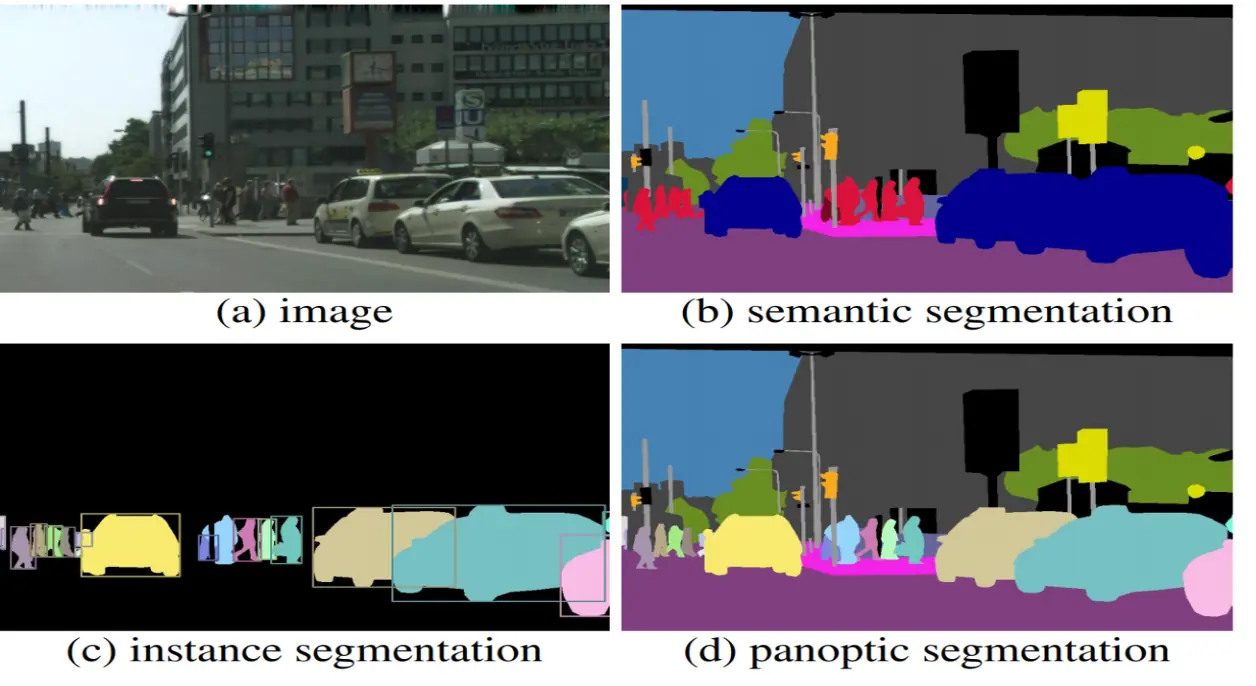
\includegraphics[width=0.9\textwidth]{semantic_vs_instance_vs_panoptic}}
  \caption{Types of segmentation.}
  \label{fig:types_segmentation}
\end{figure}

\section{Thresholding \cite{gonzalez2009digital}}
\begin{itemize}
\item Decide the classification by comparing the $I(x,y)$ pixel values with a threshold $t$, generating the binarized image
  \begin{equation}
    O(x,y) = \begin{cases*}
      1 & {\text if}\quad $I(x,y)>t$ \\
      0 & {\text otherwise}
    \end{cases*} 
  \end{equation}
  where $O(x,y)$ are the output pixel values.
\end{itemize}

\begin{figure}[H]
  \vspace{1ex}
  \centering
\href{https://github.com/vicente-gonzalez-ruiz/medical_imaging/blob/main/notebooks/thresholding.ipynb}{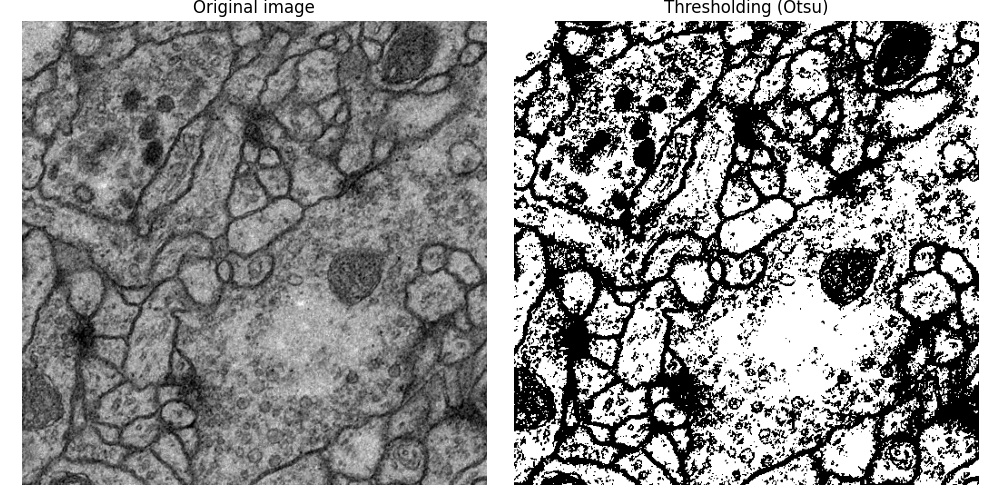
\includegraphics[width=0.9\textwidth]{thresholding}}
  \caption[An example of segmentation by thresholding.]{An example of
    segmentation by thresholding. Otsu is used for selection the
    threshold value.}
  \label{fig:thresholding}
\end{figure}

\section{U-Net segmentation \cite{ronneberger2015u}}

\begin{itemize}
\item A machine learning technique based on a deep \gls{CNN} (see Section~\ref{sec:}).
\item Supervised learning (the training set must be labeled).
\end{itemize}

%\href{https://github.com/byrkbrk/unet-implementation?tab=readme-ov-file}{unet-implementation}

%\begin{center}
%  \href{https://github.com/vicente-gonzalez-ruiz/medical_imaging/blob/main/notebooks/unet_cell_data.ipynb}{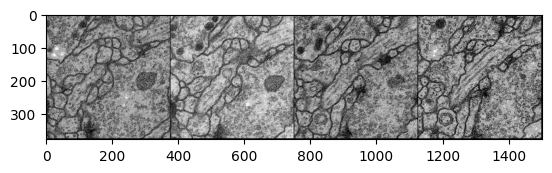
\includegraphics[width=12cm]{unet_cell_data}}
%  \href{https://github.com/vicente-gonzalez-ruiz/medical_imaging/blob/main/notebooks/unet_cell_data.ipynb}{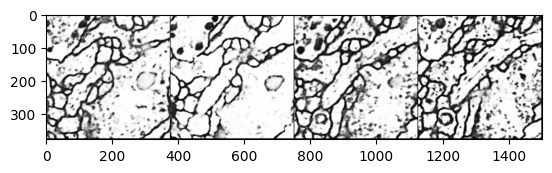
\includegraphics[width=12cm]{unet_cell_data_result}}
%\end{center}

\begin{figure}[H]
  \vspace{1ex}
  \centering
\href{https://github.com/vicente-gonzalez-ruiz/medical_imaging/blob/main/notebooks/unet_cell_data.ipynb}{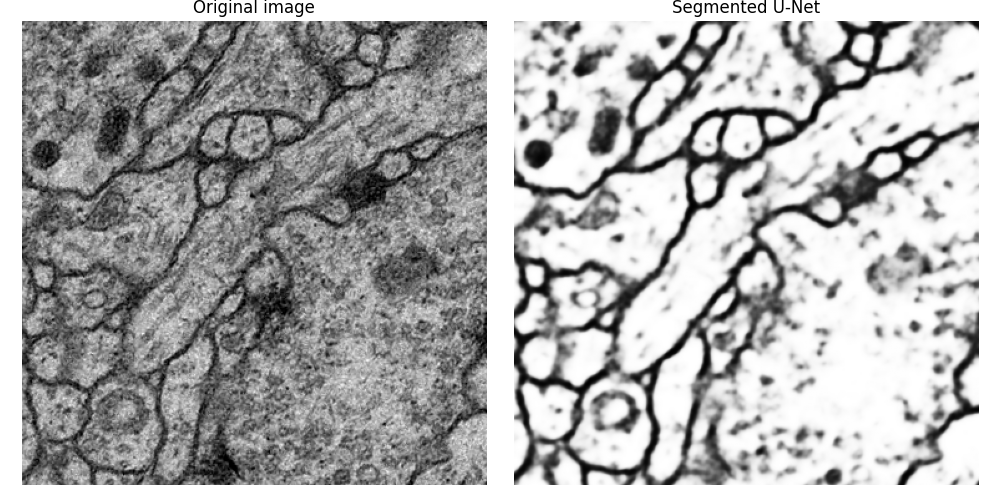
\includegraphics[width=0.9\textwidth]{U-Net_segmentation}}
  \caption[An example of segmentation using a U-Net.]{An example of
    segmentation using a U-Net. Only a crop is show.}
  \label{fig:U-Net_segmentatin}
\end{figure}



\printglossary[type=\acronymtype]

\section*{Resources}

\bibliographystyle{plain}
\bibliography{tomography,MRI,denoising}

\end{document}